\documentclass[language=english,version=final,mainfont=none,sharelatex=true,minted=true]{utuftthesis}
\setcounter{secnumdepth}{2}
\setcounter{tocdepth}{2}
\usepackage{float}
\usepackage[caption=false]{subfig}
\usepackage{graphicx}
\usepackage{listings}
\usepackage{csvsimple-legacy}
\usepackage{longtable}

\graphicspath{ {./images/} }

% Define the algorithm environment
%\makeatletter
\providecommand\textquotedblplain{%
  \bgroup\addfontfeatures{Mapping=}\char34\egroup}
\providecommand{\tabularnewline}{\\}
\floatstyle{ruled}
\newfloat{algorithm}{tbp}{loa}
\providecommand{\algorithmname}{Algoritmi}
\floatname{algorithm}{\protect\algorithmname}
%\makeatother

% allow algorithms to break pages
\makeatletter
\newenvironment{breakablealgorithm}
  {% \begin{breakablealgorithm}
   \begin{center}
     \refstepcounter{algorithm}% New algorithm
     \hrule height.8pt depth0pt \kern2pt% \@fs@pre for \@fs@ruled
     \renewcommand{\caption}[2][\relax]{% Make a new \caption
       {\raggedright\textbf{\fname@algorithm~\thealgorithm} ##2\par}%
       \ifx\relax##1\relax % #1 is \relax
         \addcontentsline{loa}{algorithm}{\protect\numberline{\thealgorithm}##2}%
       \else % #1 is not \relax
         \addcontentsline{loa}{algorithm}{\protect\numberline{\thealgorithm}##1}%
       \fi
       \kern2pt\hrule\kern2pt
     }
  }{% \end{breakablealgorithm}
     \kern2pt\hrule\relax% \@fs@post for \@fs@ruled
   \end{center}
  }
\makeatother

\addbibresource{bibliography.bib}

% baselinestrechillä voi säätää koodirivien riviväliä
\setminted{
breaklines,
baselinestretch=1,
linenos
}

\begin{document}

\pubyear{2022}
\pubmonth{11}
\publab{Ohjelmistotekniikka}
\publaben{Software Engineering}
\pubtype{M.Sc. Tech. Thesis}
\title{Storing encrypted patient data in a public cloud}
\author{Konsta Purtsi}

\maketitle

\keywords{encryption, cryptography, public cloud}

\begin{abstract}
The Finnish laws on individual's data security as well as The General Data Protection Regulation (EU) (GDPR) are legislations requiring caution from an organization handling private data.
A healthcare organization is required to exercise extreme caution when handling health data as the GDPR considers individual's health data ''a special category of personal data'', as it is sensitive by nature.

Public cloud providers such as Google Cloud Platform promise to make developing and hosting web applications simpler.
However trusting a third party such as Google with individual's health data increases the requirements for security.
The developer may want to implement additional security measures on top of those provided by default by the cloud provider. Modern cryptographic algorithms use keys to encrypt and decrypt data. However, storing the keys in a secure and performant way is no simple task.

This thesis includes an implementation of a server application built to mimic a real world application for handling patient data.
The application is built with TypeScript and hosted in Google Cloud Platform's services.
The application is used to analyze the added complexity and performance deficit of implementing strong encryption.

The complexity and performance differences with the application in encrypted mode are notable.
However, a lot of the complexity can be mitigated with good design.
No complex cryptographic algorithms have to be understood by the developer to be able to implement strong encryption.
Existing tools and libraries handle most of the work.
\end{abstract}


% mandatory
\tableofcontents

\begin{comment}
% if you want a list of figures
\listoffigures

% if you want a list of tables
\listoftables

% if you want a list of acronyms
\listofacronyms

\end{comment}

% change the name if the default doesn't sound right
\renewcommand{\algorithmname}{\listingscaption}


% chapters
\chapter{Introduction} \label{introduction}

The Finnish laws on individual's data security as well as The General Data Protection Regulation (EU) (GDPR) are legislations requiring caution from an organization handling private data.
A healthcare organization is required to take extreme caution when handling health data as the GDPR considers individual's health data "a special category of personal data", as it is sensitive by nature.
Healthcare organizations must comply with these regulations or face sanctions.

Public cloud providers such as Google Cloud Platform claim to reduce the work required for developing and maintaining an application.
However, organizations using a public cloud must take even higher caution when dealing with an individual's data.
The cloud providers promise proper security measures without any configuration needed.
The developer must still be cautious when storing data in a public cloud.

There are multiple strategies for designing and implementing secure web applications.
Modern cryptographic algorithms use secret keys to encrypt and decrypt data to keep it secure during storage and transit.
Building key-based encryption in the cloud is no simple task.
The keys to encrypt the data cannot be stored along with the data because of the risk of the database leaking allowing a malicious actor to gain access to the data.
However, storing the keys separate from the data might cause I/O issues on a large scale.
% Meneekö liian syvälle introluvuksi?
% Näkisin että vielä ihan sopivalla tasolla tämä kuvaus. -SR

\section{Research questions and the goal of the thesis}

The goal of the thesis is to research how the legislations in Finland affect healthcare organizations.
Both the Finnish law and the GDPR are analyzed in terms of how they affect the technical implementation of a digital service hosted in a public cloud.
The research includes a technical specification and implementation of a server application built to comply with the regulations.

Research questions of the thesis:
\begin{enumerate}
    \item What is required from a healthcare organization to comply with the Finnish law and the GDPR in terms of technical implementation?
    \item What is a strong enough encryption strategy for handling individual's health data in a public cloud?
    \item How does implementing encryption affect the complexity of an application?
    \item How does the encryption affect the performance of an application? 
\end{enumerate}

\section{Scope and research methods}

The scope of this thesis is to research and analyze how a Finnish healthcare organization should abide by the General Data Protection Regulation in the European Union and the Finnish law.
The legislations are analyzed in terms of their effect on the technical implementation of an application.

This thesis describes cloud computing generally and the Google Cloud Platform specifically in terms of handling encrypted patient data.
The application and infrastructure are built to handle the data in encrypted state in storage and in transit between the database and the server application.
Handling security between the client and the server such as authorization and authentication is outside the scope.

The application is built to match a specification close to a real world application.
The encryption strategy is decided to be secure enough for handling individual's health data.
The difference in complexity between no encryption and the implemented encryption is analyzed.

The application is also designed with a large amount of simultaneous connections in mind.
The finished application is load tested in both encrypted and unencrypted modes.
The load test results are analyzed in terms of performance difference.

\section{Structure of the thesis}

The thesis consists of background research on the topics of legislations, encryption and the technologies used.
Chapter \ref{data security} covers the legislations in effect in Finland and how a healthcare organization must comply with them.
Chapter \ref{cryptography background} covers the theory behind cryptography and how it can be used in a secure web application.
Chapter \ref{technologies introduction} introduces the technologies used in the conducted research.
Chapter \ref{technical analysis} lists the technical requirements of the application and the architectural design, technology choices and encryption strategy used.
Chapter \ref{technical implementation} goes through the technical implementation of the application and the infrastructure.
Chapter \ref{effect of encryption} analyses the effect of implementing encryption on the complexity of the program code and the infrastructure as well as the performance of the application.
Chapter \ref{conclusion} summarizes the thesis and discusses options for improving the application as well as options for further research.

\chapter{Patient data in a public cloud} \label{data security}

This chapter covers laws effective in Finland on storing individual's health data.
The jurisdiction is analyzed from the point of view of a healthcare provider storing patient data in a public cloud.
The laws are analyzed more by their technical requirements rather than their juridical ones.

\section{Patient data security laws in Finland}

The Finnish law includes multiple legislations to follow when storing patient data.
The main laws on this topic are for example Data Protection Act\footnote{Tietosuojalaki} 1050/2018, Act on the Status and Rights of Patients\footnote{Laki potilaan asemasta ja oikeuksista} 785/1992 and Act on the Electronic Processing of Client Data in Healthcare and Social Welfare\footnote{Laki sosiaali- ja terveydenhuollon asiakasti- etojen sähköisestä käsittelystä} 784/2021.
The main legislation to follow on data protection in Finland, which the Finnish laws complement and expand on, is the General Data Protection Regulation of the European Union.
\cite{valvira}

The General Data Protection Regulation (EU) (GDPR) is a regulation on data protection and security in the European Union (EU).
GDPR applies to all enterprises storing the data of an individual living inside the European Economic Area (EEA), regardless whether the processing itself takes place in the Union.
GDPR aims to protect individuals' data and enhance their control over it, while also making the regulation simpler to follow for companies.
\cite{gdpr}

\section{Technical requirements of the laws in Finland}

The GDPR requires the data controller --- an organization that collects data from EU residents --- to provide the individual with information and options.
The GDPR also gives some specifics on how to handle the data securely.
Many of these mandates may be fulfilled using technology.
\cite{gdpr}

The GDPR mandates that the data controller is responsible for notifying the user and collecting consent before collecting any personal data.
The individual must explicitly give consent for example by ticking a box. Silence, inactivity or pre-ticked boxes do not count as consent.
The consent must also be stored in a way that the data controller can prove that they have collected it.
\cite{gdpr}

After collecting consent, the individual has the right to know whether their data is being processed.
The consent may also be given or withdrawn at any time at will.
It should be just as easy to withdraw consent as it is to give it.
At the point the data is collected, the user must be informed of the time period the data will be stored.
If the data is no longer needed for the purpose it was collected for, it should be deleted.
The data controller must also provide a copy of the individual's data when requested.
The exported data must be in ''a structured and commonly used and machine-readable'' format.
\cite{gdpr}

The GDPR also mandates a right to be forgotten for the individual.
This means the individual can request the removal of all data concerning him or her.
The individual may also request the data to be transferred to another data controller.
The controller must oblige to these requests without any undue delay.
\cite{gdpr}

Collecting parental consent is also required by the GDPR.
Child age is defined by the specific member state, in the GDPR regulations the default being 16 years. \cite{gdpr}
In the case of Finland the specific age is 13 years \cite{tietosuojalaki}. 
In Finland, a child can use advisory, support or preemptive services without their parent's consent \cite{tietosuojavaltuusto}.

Handling a Finnish resident's social security number\footnote{Sosiaaliturvatunnus} (SSN) is regulated by The Data Protection Act.
Permission for processing the individual's SSN is granted for identification of the individual for legal purposes, such as healthcare.
The SSN must not be printed redundantly on any documents.
\cite{tietosuojalaki}

The GDPR specifies some guidelines on data security.
While not too technical, these guidelines give organizations good pointers on how to handle data.
Data security standards should be judged on a per-case basis, but some of the things the GDPR suggests are \cite{gdpr}:
\begin{itemize}
    \item the pseudonymization and encryption of personal data;
    \item the ability to ensure the ongoing confidentiality, integrity, availability and resilience of processing systems and services;
    \item the ability to restore the availability and access to personal data in a timely manner in the event of a physical or technical incident;
    \item a process for regularly testing, assessing and evaluating the effectiveness of technical and organizational measures for ensuring the security of the processing.
\end{itemize}

The data security measures can be confirmed appropriate by following an approved code of conduct or by an approved certification mechanism.
Each member state should provide a public authority to supervise GDPR compliance.
This supervisory authority has a broad and sweeping power over data controllers' activities.
\cite{gdpr}
In Finland, this supervisory authority is The Office of the Data Protection Ombudsman\footnote{Tietosuojavaltuutetun toimisto}. \cite{tietosuojavaltuutettu}

\section{Requirements for storing patient data}

The GDPR is very far from actual technical implementation, and only suggests the developer to consider the pseudonymization and encryption of personal data regarding the implementation.
The GDPR suggests considering the level of security required for data storage based on the nature of the data as well as the risks related to any incidents.
An individual's health data is considered "a special category of personal data" so the developer should take extreme caution when dealing with said data, as it is sensitive by nature.
\cite{gdpr}

Complying with the GDPR regulations will take a fair amount of technology, even if just for the bookkeeping.
Not only must data controllers make individuals’ personal data transparent and editable, they must make records of the individuals’ wishes available to supervisory authorities or else face sanction.
Any of these failures is punishable by a significant fine. \cite{gdpr}
\begin{itemize}
    \item Failure by a Controller or Processor, or their representative, to provide information on request to a supervisory authority required for the performance of their tasks.
    \item Failure by a Controller or Processor to provide access to all personal data or information necessary for performance of supervisory authority tasks.
    \item Failure to allow access to premises, including any data processing equipment.
    \item Failure to comply with an order to comply with an individual's requests.
    \item Failure to comply with an order to bring processing in to compliance in a specified manner and in a specified period.
    \item Failure to comply with an order to communicate a personal data breach to individuals.
    \item Failure to comply with a prohibition on processing.
    \item Failure to comply with an order to rectify, restrict, or erase data and to notify 3rd parties of such actions.
    \item Failure of a Certifying Body to comply with an order to cease issuing certifications.
    \item Failure to comply with an order to cease transfers of data to 3rd countries or an international organization.
\end{itemize}

Validating the privacy practices of an organization GDPR-compliant is not a well-defined task.
GDPR says to follow a code of conduct, but such codes are hard to come by.
Getting a certification from a supervisory authority is another way to validate an organization's GDPR compliance.
\cite{gdpr}

\section{GDPR compliance in a public cloud}

Public cloud is characterized by providing computation, storage \& networking services outside of one's current organization.
It also offers near infinite scalability and on-demand deployments at an inexpensive price.
Companies have adopted the public cloud at a fast speed in recent years – a trend that is probably not going to be reversed.
For example, Amazon Web Services (AWS) provides cloud computing infrastructure to over 1 million organizations in 190 countries.
\cite{sevensins}

As modern computing systems focus on performance, cost-efficiency, reliability, and scalability, not many organizations give enough thought to security and privacy.
The rise of the GDPR forces organizations to face the issues on privacy and security.
Usage of a public cloud complicates these problems even more, as multiple organizations can share computing and networking resources.
\cite{sevensins}

While a multitenant cloud has a lot of benefits for the organization using it, sharing a virtualized pool of computing and networking services is also a possible cause for security issues.
When multiple organizations share the same resource, it is a lot more likely for personal data to leak or for an unauthorized party to gain access to the data.
Public cloud providers' lack the tools required to monitor and audit these types of security issues, and leave a lot of the problems for the developer to deal with.
\cite{cloudauditing}

Right to be forgotten is not a simple task to adhere to in the real world.
Not only must all manually collected backups be cleared of the individual's data, the cloud provider may also have taken copies of the data for performance, security and scalability reasons.
Google reports that their cloud services can take up to 180 days to get the data fully deleted.
\cite{sevensins}

Cloud services are quite opaque in terms of where the data is being processed.
The individual might not know where their data is sent when using such services.
This is especially a problem for multi-layer cloud services, where parts of the infrastructure might be handled by an entirely separate cloud services, for purposes such as handling payments and collecting analytics.
The GDPR requires organizations using cloud to solve this issue by giving precise information on where the individual's data is being sent when asking for consent.
Knowing where the data is handled might not be clear to the developer either.
\cite{sevensins}

Public cloud services do also provide quite a few tools for hardening a service for better privacy and security.
Cloud providers allow separating resources into virtual private networks with configurable firewalls between the network and other resources inside the cloud or the internet.
Public cloud also has tooling for implementing for example public key cryptography and Google Cloud encrypts all data stored on their cloud storage at rest by default. 
\cite{googlecloud}

\chapter{Background on cryptography} \label{cryptography background}

The Finnish Data Protection Act and the GDPR regulate the controller and processor of any personal data to implement proper technical and organization measures in terms of security, while taking into account the level of risk related to the nature of the data stored.
Health related data is considered a special category of personal data by the GDPR and therefore should be handled with extra caution.
The GDPR mentions pseudonymization and encryption of personal as options for improving the security of sensitive data.
As health data is considered very sensitive, appropriate cautions should be taken when storing and processing it, including the two tools mentioned by the GDPR.
\cite{gdpr}

This chapter explains the basics of cryptography, unfortunately this requires a small bit of mathematics.
Different cryptographic systems are also introduced here, as well as options for implementing cryptography in a public cloud.

\section{Cryptography}

Cryptography is the science of keeping messages secure.
Encryption is a part of cryptography which in layman's terms means sending text in the form of secret writing.
The message to be sent is first converted into an indiscernible form via cryptographic methods.
The original message is called the plaintext and the encrypted message is called the ciphertext.
The message is then delivered over computer networks.
The receiver then reverses the ciphertext using the reverse of the same cryptographic method, resulting in the exact same message that was sent by the sender.
Using cryptography only the sender and the receiver can read the original message and no third party can intercept it or tamper with it on the way.
\cite{applied-crypto}

The main job for cryptography is to achieve the following traits: confidentiality, integrity and availability.
These concepts are often referred to as the CIA triad.
The meaning for each of them is the following: \cite{crypto-principles}
\begin{itemize}
    \item Confidentiality: Only the original sender and the recipient can read the message.
    No third party can eavesdrop on the communications.
    \item Integrity: The message is transmitted through the communication channel as-is without any third party tampering with it.
    \item Availability: The information is readily available without unnecessary delays to all authorized parties.
\end{itemize}

The three previously discussed concepts of cryptography are visualized in Fig \ref{fig:cryptography-concepts}.

\begin{figure}[!htb]
\centering
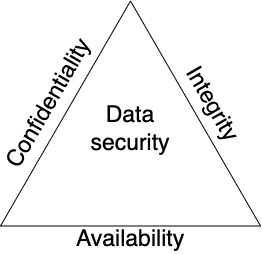
\includegraphics[scale=1.0]{cia-triad}
\caption{Visualization of the CIA triad, the three concepts of data security}
\label{fig:cryptography-concepts}
\end{figure}

The CIA triad is quite a well established list of traits.
However, some in the cryptography space feel that additional concepts are necessary.
The additional concepts often listed are the following \cite{crypto-principles}:
\begin{itemize}
    \item Authenticity: The message can be confirmed authentic using cryptographic measures.
    The users communicating are also validated as who they claim to be.
    \item Accountability: The actions of an individual are traceable to them.
    Because no system is truly secure, it is beneficial to be able to trace the source of a possible security breach.
\end{itemize}

A cryptographic algorithm, also called a cipher, is a mathematical function used for encrypting and decrypting a message.
There are often two separate functions: one for encrypting and the other for decrypting.
\cite{applied-crypto}

A cryptographic algorithm which encryption is based on keeping how the function works a secret is called a restricted algorithm.
Restricted algorithms have been used historically, but they are quite inadequate by today's standards.
If the secret is revealed at any point, every user must change to an entirely new algorithm.
\cite{applied-crypto}
% security by obscurity

Modern cryptographic solutions solve this problem using keys.
This key can be any value on a large range of values, called the keyspace.
Both operations, encryption and decryption, use this key as part of the function.
Some algorithms use a different encryption and decryption keys.
The security of these algorithms is based entirely on the secrecy of the key or keys.
The details of the algorithm can therefore be made public and analyzed.
Leaking of the algorithm is no longer an issue, as long as the eavesdropper does not gain access to the keys.
\cite{applied-crypto}

Cryptographic algorithms can be divided into two general categories: symmetric and asymmetric, also known as public-key.
An algorithm being symmetric means that the encryption key can be calculated from the decryption key and vice versa.
In most cases, the encryption and decryption key is the same.
Before beginning secure communication on a single-key algorithm, the sender and receiver must agree on a key.
The key is central to the security of the communication, keeping it a secret makes the communications a secret.
\cite{applied-crypto}

Public-key algorithms are characterized by using a separate key for both encryption and decryption.
The decryption key cannot be calculated from the encryption key (in a reasonable time).
The encryption key is often called the public key.
The decryption key is referred to as the private key.
The algorithms are named "public-key" because the encryption key can be made public.
Anyone can use the public key to encrypt a message, but only a specific person with the private key can decrypt it.
It is also possible an algorithm uses the private key to encrypt and the public key to decrypt data.
An example of such use case would be digital signatures, which prove a specific person's signature to be genuine and the authenticity and integrity of the message.
\cite{applied-crypto}

The most relevant public-key algorithms use prime numbers as the basis of their functionality.
The primes used are very, very large: many hundred digits long.
\cite{practical-crypto}
Factoring a number means finding its prime factors.
The core idea in using primes in cryptography, is that factoring a number is very time-consuming.
For example, in 1993 a 120-digit hard number was factored in 3 months of real time using 825 mips-years\footnote{
Mips-year is an unit used to measure computational effort in cryptography.
One mips-year is the amount of work performed by a single computer in a year, operating at one million operations per second or 1 MIPS.
}
of computing power.
On the other hand, generating prime numbers and multiplying them is easy.
Answering the question "is \textit{n} prime?" is a lot easier than answering the question "what are the factors of \textit{n}?" because the former is just a yes/no question.
\cite{applied-crypto}
Multiplication is more work than addition, for example, but it is still relatively easy for a computer to perform.
\cite{practical-crypto}

\section{Pseudonymization}

Pseudonymization means changing all identifiable personal data such as e-mail addresses, names and IP addresses for aliases.
The information can no longer be connected to a specific individual without additional data.
Pseudonymization is highly recommended by the GDPR.
Although the process of pseudonymization is reversible, it significantly lowers the risk of leaking sensitive data.
\cite{gdpr}
The irreversible process of changing identifiable personal data for an alias is called anonymisation.

The GDPR suggests organizations to implement pseudonymization, however it does not define a technique or process for it.
The GDPR only gives us the end goal of pseudonymization: making the data unable to be attributed to a natural person.
By this definition, encryption fulfills this goal.
\cite{pseudonymisation}

% Voi miettiä, meneekö vähän syvemmällekin vaikkapa esimerkin kautta
%

\section{Envelope encryption}

Envelope encryption is an encryption strategy used with large scale applications.
It allows for both, centralized safekeeping of encryption keys as well as encrypting a large amount of data.
Envelope encryption uses multiple layers of keys by encrypting a key with another key.
The key that is used to encrypt another key is called the \textit{key encryption key} (KEK).
The key that encrypts the data itself is called the \textit{data encryption key} (DEK).
The process of decrypting a DEK with a KEK is also called wrapping, and is visualized in \ref{fig:envelope-encryption-key}.
Decrypting the data with the DEK is visualized in \ref{fig:envelope-encryption-data}.
\cite{googlecloud}

Google lists best practices for working with DEKs and KEKs.
DEKs should be generated locally by the program handling the data and always encrypted at rest.
For easy access, the DEK can be stored near the data it encrypts.
KEKs should be managed and stored centrally, for example on Google Cloud Platform's Cloud Key Management Service (KMS).
The granularity of KEKs should be considered by workload, the same KEK can be used for data the workload is responsible for.
KEKs should be rotated regularly and also after any suspicious activity.
A new DEK should be used every time new data is stored.
This also means DEKs will never have to be rotated.
The same DEK should never be used for two different users.
\cite{googlecloud}

The security advantage of envelope encryption is in the key encryption key and using a different data encryption key for each chunk of data.
Even if a malicious actor were to gain access to a plaintext DEK, they would only be able to decrypt a small chunk of data.
The malicious actor would need both: the centrally stored KEK as well as the database with the DEKs to decrypt all the data.
\cite{googlecloud}

\begin{figure}[!htb]
\centering
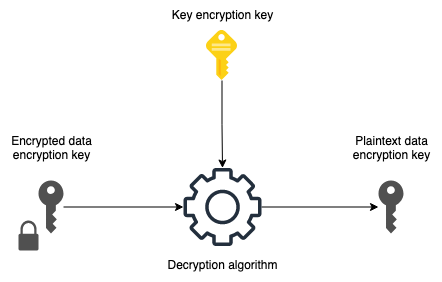
\includegraphics[scale=0.8]{envelope-encryption-key}
\caption{Visualization of decrypting a data encryption key with a key encryption key}
\label{fig:envelope-encryption-key}
\end{figure}

\begin{figure}[!htb]
\centering
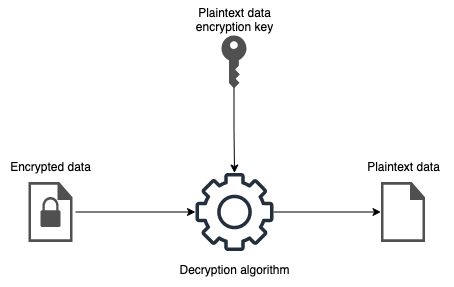
\includegraphics[scale=0.8]{envelope-encryption-data}
\caption{Visualization of decrypting data with a plaintext data encryption key}
\label{fig:envelope-encryption-data}
\end{figure}
\chapter{Introduction to the technologies used} \label{technologies introduction}

This chapter includes introduction on the technologies chosen for the POC (proof-of-concept) project.
The technologies and their roles in the project are explained in the amount of detail necessary.

The project is built as a POC implementation of a GDPR-compliant patient data storage for a healthcare organization.
The technologies are chosen after evaluating their fit for the project and their familiarity for the organization after discussing the choice with them. 
The chosen technologies are as follows:
\begin{itemize}
    \item Google Cloud Platform
    \item Terraform
    \item PostgreSQL
    \item Node.js
    \item TypeScript
    \item Docker
\end{itemize}

\section{Google Cloud Platform}

There are many providers in the cloud computing space.
For example, Amazon, Google, Microsoft, Rackspace and DigitalOcean have grown to provide services for numerous users.
Different providers offer similar products, but the implementation details and how they work vary significantly.
\cite{mastering-google-cloud} 

Google Cloud Platform (GCP) is a selection of cloud computing services provided by Google.
GCP started as Google App Engine framework for hosting web applications from Google's data centers and grew from there to offer a wide variety of services.
Nowadays, it is one of the largest cloud computing platforms, but still behind Amazon Web Services (AWS) and Microsoft Azure in market share.
Google promises the users of its cloud platform 99.95 \% reliability, which they achieve by building safety systems around in their applications by assuming any of the parts can fail.
Google is also running constant performance and load tests on their services, finding and troubleshooting problems proactively.
\cite{mastering-google-cloud}
Different categories of services offered GCP are visualized in Fig \ref{fig:google-cloud}.

\begin{figure}[!htb]
\centering
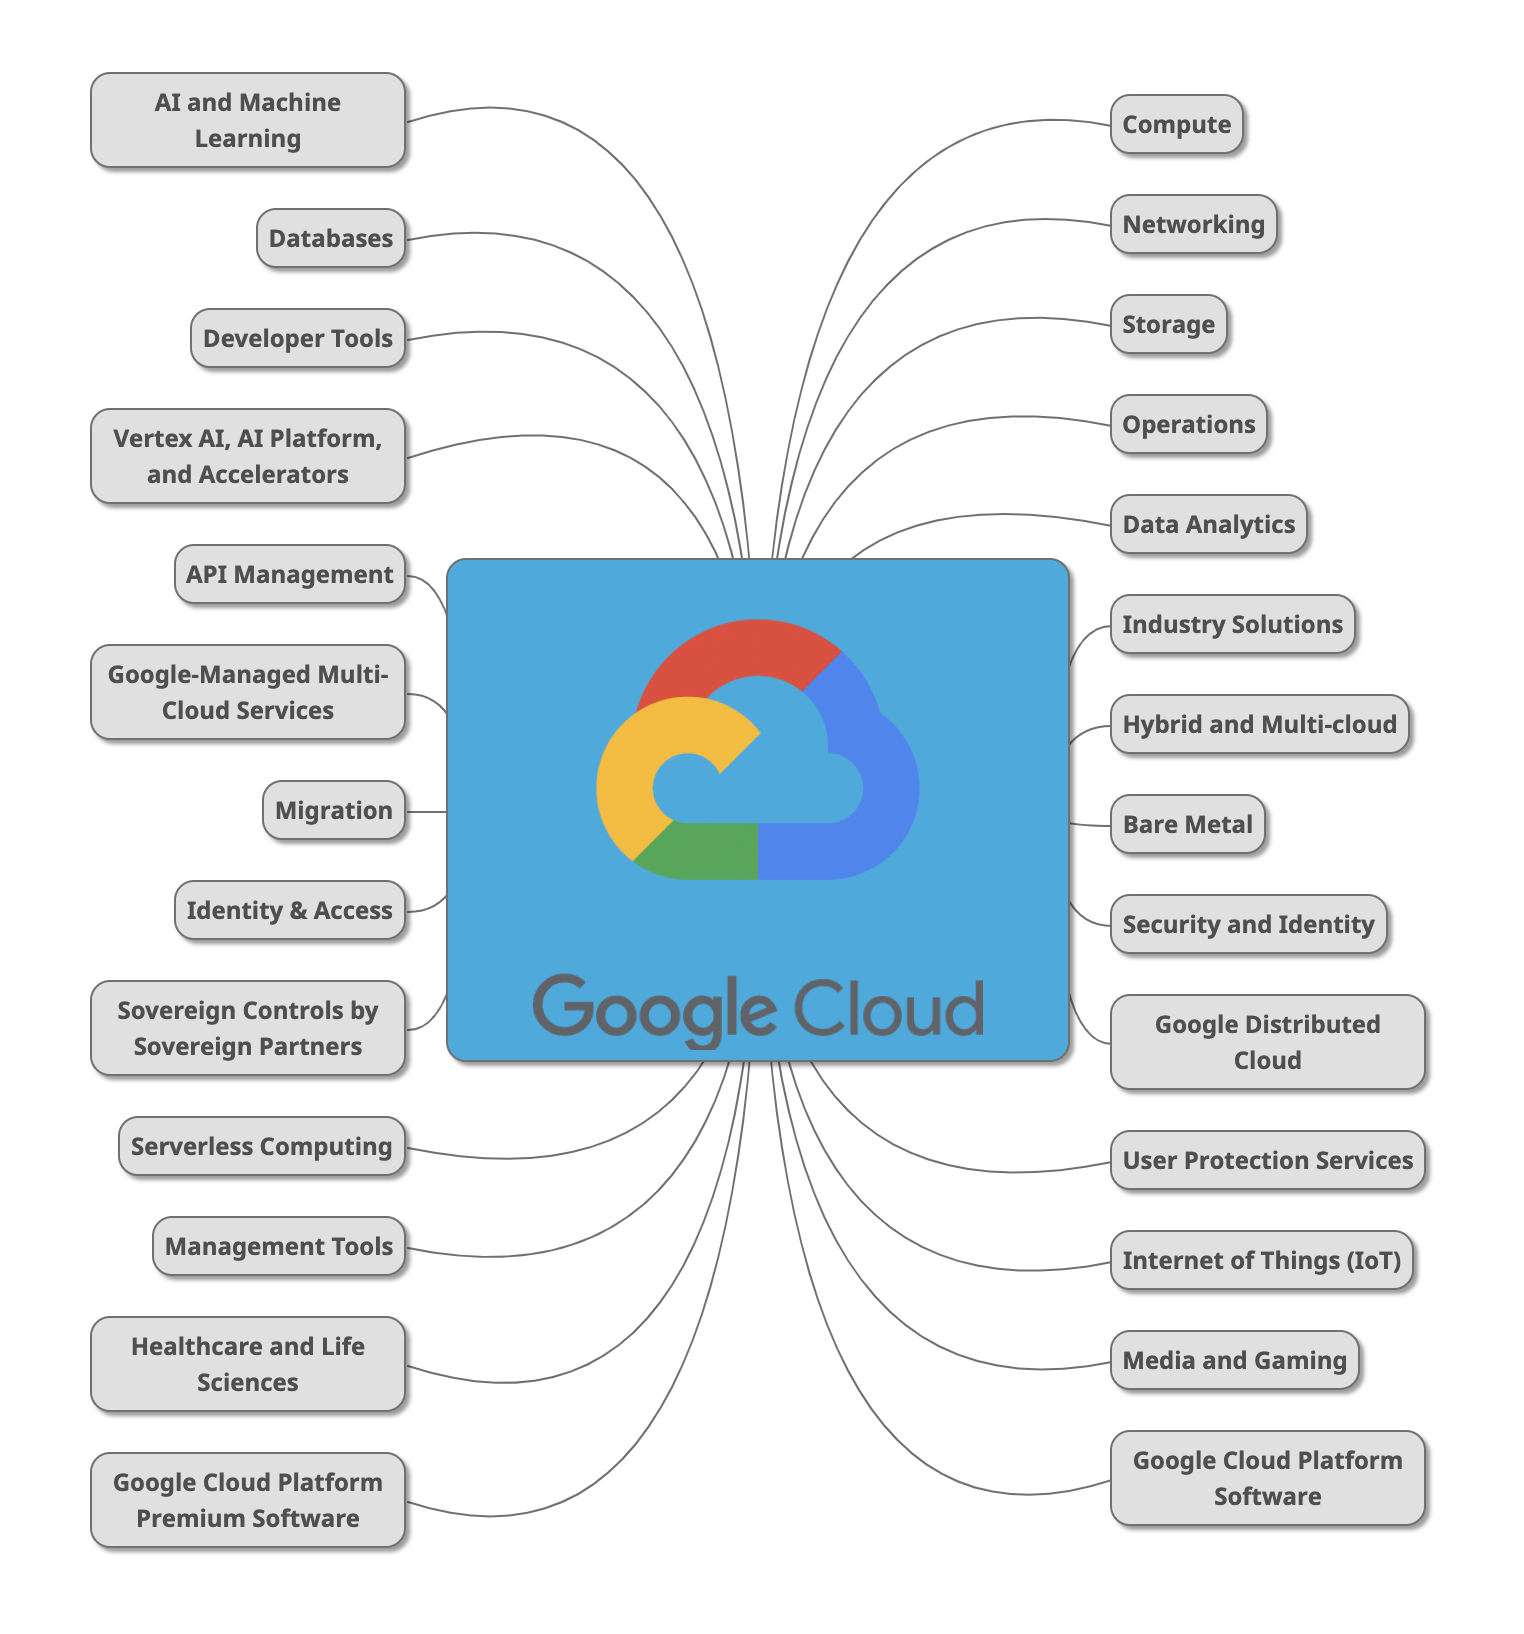
\includegraphics[scale=0.55]{googlecloud}
\caption{Visualization of the categories of services Google Cloud Platform offers}
\label{fig:google-cloud}
\end{figure}

The most straightforward way to manage the services provided by Google Cloud Platform is the web-based console served at console.cloud.google.com.
Google also offers tooling called the Cloud SDK for interfacing with Google Cloud Platform.
The SDK supports interacting with Google Cloud Platform products and services using client libraries for Java, Python, Node.js, Ruby, Go, .NET and PHP.
The SDK also includes a command line tool called the Google Cloud CLI for managing GCP services.
\cite{googlecloud}

Google Cloud Platform offers many options for building cloud based services.
GCP offers compute, storage and networking services along with many others.
For example, Google App Engine is a service for hosting a fully managed server-side application.
Cloud SQL is Google cloud's offering for a fully managed PostgreSQL database.
Cloud DNS is their platform for managing all things DNS as well as registering and managing domains.
These are only a few examples of the services provided by Google Cloud Platform.
The specific services chosen for the POC are explained in more technical depth in the next chapter.
\cite{googlecloud}

\section{Terraform}

In place of managing cloud computing resources using a web-based console, a client library or a command line interface, there is another option.
Infrastructure as Code (IaC) is defined as building infrastructure in a declarative way.
Instead of clicking through a graphical interface or building a script to tell a computer how to build the infrastructure, IaC languages are used to define what the infrastructure is, and let the IaC technology handle building and changing it.
IaC technologies have the benefit of making the infrastructure more replicable and easier to version and document.
\cite{terraform}

Terraform is an open source infrastructure as code tool created by Hashi\-Corp.
Terraform as a technology consists of multiple tools: Terraform CLI, Terraform Cloud and Terraform Enterprise.
In the scope of this thesis, the most relevant tool is Terraform CLI: a command line tool launched using the \verb|terraform| command.
Terraform CLI can be used for any action the developer would do such as \verb|terraform plan| and \verb|terraform apply|.
Terraform uses HashiCorp's own Hashi\-Corp Configuration Language (HCL) as its main interface.
HCL aims to be both: a human- and a machine-readable configuration language for use with command line tools.
\cite{terraform}

Terraform allows building both cloud and on-premise infrastructure.
Terraform does not specialize in any technology, but instead it allows for the use of so-called providers for many different platforms and technologies.
At the time of writing HashiCorp and the Terraform community have released over 1700 different providers on the Terraform registry\footnote{https://registry.terraform.io/} including for example Amazon Web Services (AWS), Azure, Google Cloud Platform (GCP), Kubernetes, Helm and many more.
Terraform providers interface with different cloud platforms and other services via their application programming interfaces (APIs).
A provider can be created for virtually anything that has an accessible API.
\cite{terraform}

The Terraform workflow consists of three main steps.
First, the developer writes the configuration which defines the infrastructure.
The second step is the plan stage where the developer reviews the changes Terraform will make to the infrastructure, including things that will be created, updated or destroyed.
Third, the developer applies the planned changes to the actual infrastructure.
Terraform will handle changing the infrastructure in the correct order and updating its own internal state file.
Destroying the infrastructure can be considered the fourth step after the infrastructure has served its purpose.
\cite{terraform}
The Terraform workflow is visualized in Fig \ref{fig:terraform-workflow}.

\begin{figure}[!htb]
\centering
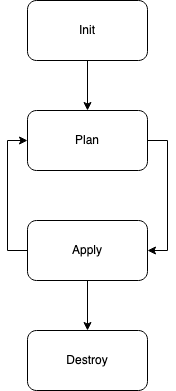
\includegraphics[scale=0.8]{terraform-workflow}
\caption{Visualization of the steps included in the Terraform workflow}
\label{fig:terraform-workflow}
\end{figure}

Terraform has an abstraction called a \textit{module}.
A module is a lightweight container that includes multiple resources that are used together.
Using a module makes declaring the architecture itself easier, without declaring the physical parts themselves.
A module can also take input variables to allow for building configurable and reusable building blocks.
It can return output values as well, which can be used as arguments elsewhere.
\cite{terraform}

\section{PostgreSQL}

PostgreSQL is an open-source object-relational database management system.
It is designed to handle a large variety of workloads ranging from single servers to data warehouses and huge web services.
It has a history spanning over 30 years which gives it a reputation as a powerful, reliable, robust and performant database.
PostgreSQL supports a large part of the SQL standard and offers many more modern features, such as complex queries, foreign keys and updatable views.\footnote{Foreign keys are used to validate the existence of an entry and store a reference to it in another database table. An updatable view is a database view that can be updated similarly to a regular table.}
\cite{postgresql}

PostgreSQL is based on a database system developed at the University of California at Berkeley Computer Science Department: POSTGRES, Version 4.2.
POSTGRES pioneered many new concepts for database systems.
PostgreSQL is an open-source successor of POSTGRES.
It is released under a very liberal license allowing for use in any sort of application, be that private, commercial or academic.
\cite{postgresql}

The PostgreSQL database runs on macOS, Windows, Linux, FreeBSD and Open\-BSD. \cite{postgresql}
In addition to running PostgreSQL on the user's own server hardware, many cloud providers sell managed services for hosting PostgreSQL.
For example, The Google Cloud Platform includes a fully-managed service for hosting and administering a PostgreSQL database called the Cloud SQL.
\cite{googlecloud}

\section{Node.js}

Node.js is a runtime environment for JavaScript which is designed to build scalable network applications.
Node.js is a cross-platform environment which can be used to run JavaScript outside the browser for use cases such as command line tools and server-side applications.
It is an open-source project built by the OpenJS Foundation and runs on Google Chrome's V8 JavaScript engine.
Node.js was first released in 2009 and has gained huge popularity among all types of users ever since.
\cite{nodejs}

Node.js uses an event-driven architecture for building applications.
It executes code concurrently, such as allowing for multiple connections.
This is in contrast to the more common thread-based model.
The concurrency model makes building scalable systems with Node.js very reasonable, as user will not have to worry about deadlocking.
However, this does not mean Node.js can not take advantage of multiple cores in your environment.
\cite{nodejs}

Node.js is designed to be modular.
It can be extended using packages installed via Node package manager (npm).
Npm is a command line tool designed to make installing packages quick and easy.
Npm's registry has grown to become the world's largest software registry.
The registry can be browsed using its website at https://npmjs.com.
\cite{npm-docs}

Express is a web framework for Node.js.
It is designed to be fast, unopinionated and minimalist.
Express makes building solutions such as APIs for web and mobile applications simple and flexible.
Express by itself only includes a thin layer of web fundamentals required, but it can be expanded with any of Node.js libraries.
Requests to the Express application can also be intercepted and handled with a method called \textit{Middleware}.
\cite{expressjs}

Pg-promise is another example of a Node.js library built to interface with PostgreSQL.
It is built on top of node-postgres.
The name pg-promise comes from it only first adding promises as its sole feature, JavaScript's solution for handling asynchronous computation.
Nowadays the library adds a lot of other features as well.
The features it adds include for example automatic connections, automatic transactions and improved query formatting.
\cite{pg-promise}

\section{TypeScript}

TypeScript is a programming language created by Microsoft.
TypeScript extends JavaScript's syntax by adding types to it.
It is a strict superset of JavaScript, which means all existing JavaScript code is also valid TypeScript code.
JavaScript already provides primitive types such as string and number, but does not do any type checks with these.
TypeScript allows describing types explicitly and inferring types from constants.
The compiler then checks for type errors before ever running the code.
TypeScript promises to give the developer better tooling such as tighter integration with the editor.
It also promises to allow for finding bugs earlier on in the development.
\cite{typescript}

TypeScript compiles to JavaScript and can run anywhere JavaScript runs. The possible execution environments include for example web browsers and Node.js.
JavaScript already uses types such as \texttt{string} and \texttt{number}, but it does no checking on how variables are assigned.
TypeScript does this and allows defining more complex types.
\cite{typescript}

TypeScript uses all the same types JavaScript already has, but also adds a few more.
For example, the \texttt{any} type allows anything to pass into the variable.
TypeScript also has support for defining more complex types.
An \texttt{interface} can be used to define the shape of an \texttt{object}.
The \texttt{type} syntax can be used to create even more specialized types, such as unions and \texttt{string} or \texttt{number} literals.
\cite{typescript}
An example of defining types in TypeScript is shown in Listing \ref{typescript-example}.

\begin{breakablealgorithm}
\caption{An example of definining types in TypeScript.}
\label{typescript-example}
\begin{minted}{typescript}
// define the shape of a student object.
interface Student {
    name: string;
    startYear: number;
}

// union of number and string
type NumberOrString = number | string;

// union of OS's as string literals
type OS = 'Windows' | 'Linux' | 'MacOS';
\end{minted}
\end{breakablealgorithm}

TypeScript also adds syntax for defining generics similar to languages like Java and C\#.
Generics are used to provide types as variables to either other types or functions using angle brackets \texttt{<>}.
For example, generics are used to define what type of contents an array has.
\cite{typescript}
An example of using generics is shown in Listing \ref{typescript-generics}.

\begin{breakablealgorithm}
\caption{An example of using generics in TypeScript.}
\label{typescript-generics}
\begin{minted}{typescript}
// An array that takes only strings
type StringArray = Array<string>;

// A generic function for creating a tuple of any type.
function duplicate<Type>(arg: Type): [Type, Type] {
    return [arg, arg]
}
\end{minted}
\end{breakablealgorithm}

\section{Docker}

Docker is a software development tool built to make the same software run anywhere regardless of the infrastructure.
Docker can be used for all steps in the software delivery pipeline: developing, testing, shipping and running the software.
Docker promises to shorten the gap between development and production.
\cite{docker}

Docker packages and runs applications in a loosely isolated environment called a \textit{container}.
Containers are lightweight and self-contained so no other requirements other than installing Docker itself are set on the host system.
This also allows sharing containers between different users and machines without changing how the container functions.
When ready, the application can be deployed as a container or an orchestrated service.
The application works the same regardless of where it is hosted: a local server, a cloud provider or a hybrid between the two.
Docker also allows for responsively scaling of infrastructure due to its portable and lightweight nature.
\cite{docker}

an \textit{image} is a read-only template with instructions on how to create a Docker container.
An image is often based on another base-image, such as  the \texttt{ubuntu} image, with additional customizations on top.
The customizations often include building and running a custom-built application.
A custom Docker image is created with a simplistic \texttt{Dockerfile} format.
\cite{docker}

A Docker \textit{registry} stores Docker images.
When using \texttt{docker run} or \texttt{docker pull} commands, the required images are downloaded from the registry of choice.
Docker Hub is the public registry anyone can use.
For a more private store of Docker images, a private registry can be hosted.
\cite{docker}
One cloud hosted option for this is the \textit{Artifact Registry} on the Google Cloud Platform.
\cite{googlecloud}

\chapter{Technical analysis} \label{technical analysis}

This chapter explains the technical requirements for the POC (proof-of-concept) project, which is central to the analysis of the research question of the thesis.
The chapter also lists our options for the technical implementation as well as rationalizes the decisions made.

\section{High level specification}

% datan voi pitää PoC:ssa yksinkertaisena, esimerkiksi asiakkaiden vastaanottoajat (nimi, hetu, pvm, vastaanottajan tiedot ja toimipisteen tiedot). Näitä sitten muutama miljoona skriptillä. 
% Kryptauksen kysymykset ovat mielestäni juuri niitä avainasioita, joita olisi työssäsi hyvä käydä läpi
% Miten luettelemasi tavat vaikuttavat suorituskykyyn, ohjelmiston ja ympäristöjen toteutukseen, ylläpidettävyyteen ja selkeyteen. 
% Tuovatko ne oikeasti lisäturvaa.
% PoC:ssa toteutettavaksi voisi valita yhden, joka paperilla osoittautuu parhaimmaksi vaihtoehdoksi.
% Tai sitten tekee useamman toteutuksen ja tekee kovan vertailun. Ihan miten ajakäyttöösi ja työsi rakenteeseen vain parhaiten sopii.

The POC projects is built to replicate a close-to real world application for storing sensitive customer data.
The data stored is related to appointment times of any specific customer.
The application must be able to receive new appointment times and save them persistently.
It must also be able to load the state of the appointments.
All the actions are required to be fulfilled in a timely manner.
The appointment must store at least the following data
\begin{itemize}
    \item The customer's name
    \item The customer's social security number
    \item Date and time of the appointment
    \item Practitioner's name and basic info
    \item Location's name and basic info
\end{itemize}

The application must be available on the web and use an existing standard for interfacing with it.
Additional technical specifications are discussed in the next section.

\section{Technical specifications}

The application must support reading and writing data on practitioners and customers' appointments.
Preferably, the application provides REST-like endpoints for both types of data.
Each appointment must reference exactly one practitioner to whom the appointment is reserved.
All the data the application saves must be stored in a persisting PostgreSQL database.

The application must encrypt all data before it is sent to the database i.e. encryption at rest.
The master key for decrypting the data must be stored in a secure place, preferably inside the cloud provider's pre-made solution.

The application must be hosted inside the Google Cloud Platform's offering.
The products used can be chosen freely while considering the most practical option for the task, while preferring fully-managed options.

After the technical implementation of the application and the infrastructure are built, the performance of the application will be benchmarked with both encryption enabled and disabled.
This is likely to expose bottlenecks of the system, which will then be analyzed further to improve the performance of the application.

% Toteutuksen selkeys ja ylläpidettävyys tähän?
% Kuuluuko tekniseen speksiin vai tutkimuskysymykseen?

% Kirjottasko tähän miksi valittiin tietyt tekniikat?


% Mielestäni tähän sopivat syyt tekniikkojen valinnoille, voi toki olla myös oma alilukunsa tai sitten voi lisätä tämän aliluvun otsikkoon "and architectural decisions" tms.
% 
% Jos selkeydellä ja ylläpidettävyydellä viitataan näiden laatuattribuuttien arviointiin, niin tämä voi olla ehkä myöhemminkin?
%
% -SR

\section{Technology and architecture decisions}

The technological and architectural decisions are explained in this section.
The decisions were based on the specification of the POC project and based on solutions most commonly used in the industry.

The server application will be built with TypeScript running on top of Node.js.
TypeScript is a well-proven language for writing business critical applications using Node.js' large ecosystem of packages.
As the basis for the RESTful application, we will use Express: a minimal framework for building web applications.
The database for storing our patient data will be PostgreSQL.
The interface library for our database is pg-promise.
These technologies were selected because of their use in the business as well as their match with our specification.

Docker is used during development for ease of spinning up a local PostgreSQL database for development.
The server application will also be built into a custom Docker image for production.

For hosting the POC project we have decided to use Google Cloud Platform and its solutions most compatible with our technology requirements.
For hosting the Node.js application, GCP's \textit{Cloud Run} will be used.
Cloud Run is a fully-managed service for running containerized applications.
For hosting our application's Docker images, we will use GCP's \textit{Artifact Registry}.
Artifact Registry is a cloud-based solution for managing a Docker registry.
For managing our PostgreSQL database, GCP's \textit{Cloud SQL} is the technology of choice.
Cloud SQL is a fully-managed service for administering relational databases, and it supports PostgreSQL along with MySQL and SQL Server.

For managing our sensitive environment variables, GCP's \textit{Secret Manager} is the service selected.
Secret Manager promises to store sensitive secrets encrypted and secure.
For secure encryption and decryption of data, without customer accessible keys, we will use GCP's \textit{Cloud Key Management}.
The encryption strategy will be discussed in more detail in the coming sections.

For a real world use case, we might also need solutions for managing routing, domains and virtual private networks.
In our POC project, the Cloud Run application is connected straight to the internet using the GCP provided dynamic domain.
Another part of a real world application's infrastructure not included here is a user management solution.
This is also outside the scope of the POC project.
The infrastructure is visualized in figure \ref{fig:infrastructure}.

\begin{figure}[!htb]
\centering
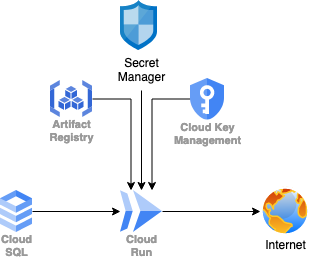
\includegraphics[scale=0.9]{infrastructure}
\caption{Visualization of the infrastructure in the Google Cloud}
\label{fig:infrastructure}
\end{figure}

\section{Cryptography options on Google Cloud}

Google Cloud Platform offers multiple solutions for encrypting data.
The easiest solution for implementing encryption with Google Cloud Platform is to let Google handle it automatically.
Google encrypts all of their customer data at rest by default, with zero configuration required by the developer.
This is done to avoid the possibility of a data breach allowing a malicious actor direct access to the plaintext data.
This encryption uses the same standards for hardened key management services that they use internally.
This system uses the AES-256 encryption standard.
\cite{googlecloud}

Besides GCP's encryption by default, developers can choose to encrypt their data with other options.
GCP's Cloud Key Management Service (KMS) is a solution for creating, using, rotating and managing cryptographic keys entirely on Google Cloud.
KMS can be used for example to provide customer-managed encryption keys (CMEK) for GCP's Cloud Storage or called by an API to encrypt any plaintext data.
Keys stored in KMS are designed to never leave Google servers making them theoretically impossible to be stolen if a malicious actor gains access to the system.
While KMS can be used to encrypt almost anything, it is built more for being the central key store in a multi-layer encryption architecture such as for storing the key encryption keys in an envelope encryption setup.
\cite{googlecloud}

GCP also provides the option for customer-supplied encryption keys (CMEK) for many of its products that encrypt data by default, such as Cloud Storage.
Google does not permanently store these type of keys, instead the key must be provided along with any operation call.
A cryptographic hash of the key is stored on Google server to validate the requests.
\cite{googlecloud}

The PostgreSQL database system has built-in support for multiple types of encryption.
A fully-managed PostgreSQL limits the developer's options a little, as they do not have access to encrypt the entire data partition by themselves.
However, encryption for specific columns using PostgreSQL's built-in pgcrypto-module is still possible.
The data can also be encrypted on the client side before it is sent to the database system.
\cite{postgresql}

% trade-off for column-level encryption:
% client can no longer query data based on that column
% workaround: hash and salt the same data and store in another column for lookups

Fully cloud-based applications cannot be considered end-to-end encrypted, as the cloud provider theoretically has access to the unencrypted data while it is processed.
The solution to this would be encrypting the data on the client-side before it is sent to the cloud provider.
This can be done either on-premises or on the user's client device.
% lähde?

\section{The encryption strategy used}

For the POC project, an additional layer of security on top of GCP's encryption by default is required to secure the patient data.
For this reason, we will encrypt all sensitive data on the server before it is written to the database.
Google Cloud Key Management System is our choice of technology for managing secrets.
However, we want to minimize the calls to the KMS API for cost reasons\footnote{Google bills us \$0.03 per 10 000 requests to the API.}
and to allow for extra scalability.
For these reasons, we will not encrypt the data itself with the KMS API, but instead employ envelope encryption.

A great option for strong implementation of envelope encryption is to have the key encryption keys never leave KMS.
The data encryption keys will be generated on the server per-request to encrypt the data itself locally.
The DEKs are encrypted using the KEKs via KMS.
This allows for calling KMS only once per fixed-length DEK instead of once per each variable-length database column to cut down the amout of KMS API calls.

In a production environment, the above option is preferred.
However, in our small-scale solution, with plans to stress test the encryption setup, the KEK will be stored encrypted in an environment variable.
% Muokkasin edeltävää virkettä, kannattaa tarkistaa -SR
The KEK will be encrypted via KMS and decrypted on application startup.
This cuts down on calling the KMS API even more and makes sure we will never be billed more than a dollar for our use of its API.
Realistically, this is also a security vulnerability, as the key has to be generated in plaintext outside KMS and is stored in plaintext inside the server application's memory.
For these reasons, this solution is not recommended for any real private and sensitive data.

The encryption of the data itself can be handled on the server application code or by the database itself via PostgreSQL's built-in pgcrypto.
For the POC application, we decided to encrypt the data on the application itself to remove the bottleneck created by having to make two queries to the database: one for the DEK and one for the data itself.
The decision was also made to allow for more research into implementing encryption.

For encrypting the data and wrapping the data encryption key, Node.js standard library's crypto-module was chosen.
This module includes a lot of useful cryptographical utilities for generating keys, and encrypting and decrypting data with multiple encryption algorithms.
\cite{nodejs}
For our POC project we will use the crypto-module for generating data keys and implementing AES-256 encryption.
We will use Google Cloud Key Management Service to decrypt our key encryption key on program startup.

\chapter{Technical implementation} \label{technical implementation}

This chapter explains the implementation of our TypeScript application and the Google Cloud infrastructure.
To fulfil the specification for our POC project, we will build a RESTful API with two resources: appointments and practitioners.
The application does not provide all of the CRUD operations (Create, Read, Update and Delete).
Only creating new resources and reading existing ones is supported.
The functionality for updating or deleting resources has not been implemented.
This is done for simplicity, as it is not needed for the scope of the analysis of this thesis.
The program code of a fully implemented application is listed in Appendix \ref{application-code} and infrastructure code in Appendix \ref{infrastructure-code}.

\section{Implementing a minimal application}

In this section, we will build an application matching the specification, except there will be no encryption just yet.
Implementing the encryption is done in the next section.

\subsection{Implementing the TypeScript application}

For the POC project, our application only serves four REST endpoints:
\begin{itemize}
    \item
    \texttt{POST /appointments/} – create a new appointment
    \item
    \texttt{GET /appointments/} – read all the appointments
    \item
    \texttt{POST /practitioners/} – create a new practitioner
    \item
    \texttt{GET /practitioners/} – read all the practitioners
\end{itemize}
The file tree of the application providing these four endpoints is visualized in Figure \ref{fig:filetree}.

\begin{figure}[!htb]
\centering
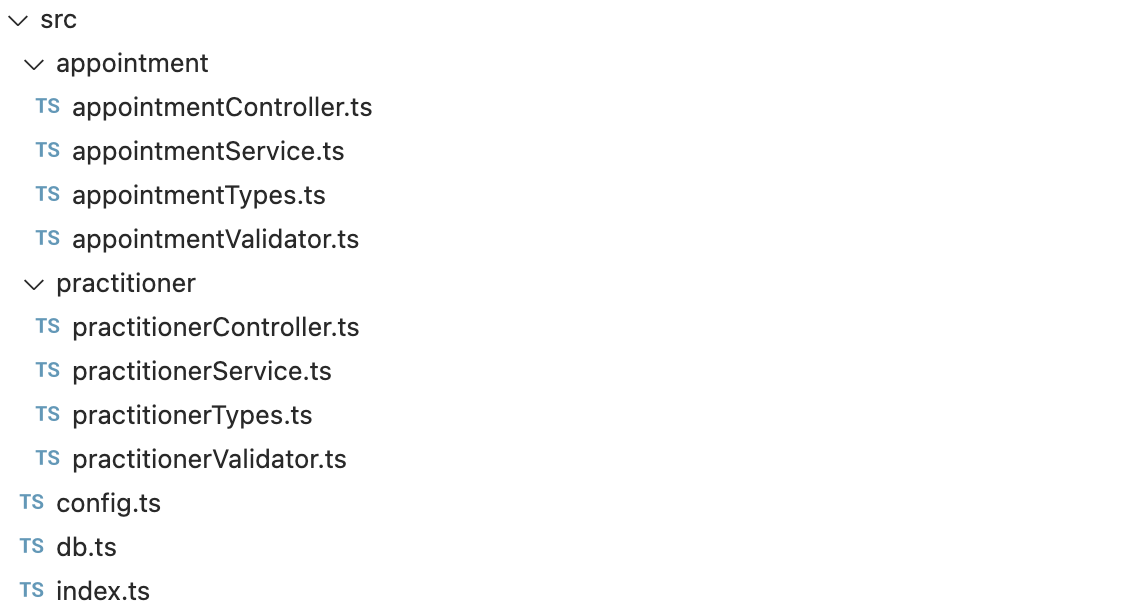
\includegraphics[scale=0.7]{filetree}
\caption{The file tree of a fully functional application}
\label{fig:filetree}
\end{figure}

The role of each file in the application can be understood via a simple request example.
For example, the following is the processing flow of a \texttt{POST /practitioners/} request:
\begin{enumerate}
    \item
    \texttt{index.ts} –
    This is where the Express-application is initialized, along with the middleware.
    From here, the request is routed to the correct controller.
    \item
    \texttt{practitionerController.ts} –
    Handles the routing for the endpoints at\\ \texttt{/appointments/}.
    First, the \texttt{validatePractitioner}-function is called, to validate the body of the request.
    Second, the \texttt{insertPractitioner}-function is called to save the new practitioner.
    \item
    \texttt{practitionerValidator.ts} –
    Validates the body of the request is an object, and it includes the required fields.
    \item
    \texttt{practitionerService.ts} –
    Executes an SQL query and inserts a new row into the database table \texttt{Practitioner}.
\end{enumerate}
A request to the \texttt{POST /appointments/} is handled very similarly, except that there is a relation between the appointment: the practitioner it is being booked for.
So, in addition to the flow explained above, the application checks that the practitioner exists.

A request to either of the \texttt{GET} endpoints does no validation for the request, as there is no body to validate.
It only queries all the rows from the database for the specified resource.

In addition to the files used to handle the request, there are two files not explained yet: \texttt{config.ts} and \texttt{db.ts}.
The former one handles the environment variable configuration in a type safe way: by throwing if the environment variable does not exist.
The latter initializes the database connection.

\subsection{Implementing the Google Cloud infrastructure}

The infrastructure for our POC project is built on the Google Cloud Platform.
It is managed by the Terraform infrastructure-as-code language.
The fully functional infrastructure is visualized in Figure \ref{fig:filetree-infra}.

% My module structure is bad. A quote from Terraform's docs:
% "We do not recommend writing modules that are just thin wrappers around single other resource types. If you have trouble finding a name for your module that isn't the same as the main resource type inside it, that may be a sign that your module is not creating any new abstraction and so the module is adding unnecessary complexity. Just use the resource type directly in the calling module instead."

The role of each notable file and module is as follows:
\begin{itemize}
    \item
    \texttt{gcp\_init.tf} –
    Declare the required version of Terraform and the providers needed.
    Initialize the Google Cloud Platform's provider with the correct project, region and zone.
    \item
    \texttt{main.tf} –
    The constants such as database configuration are declared here.
    All of the modules are are loaded and used here.
    \item
    \texttt{modules/artifact-registry} –
    Creates a private Docker repository for storing the Docker images for our server application.
    \item
    \texttt{modules/cloud-run} –
    Creates and configures a Cloud Run service to run our containerized server application. 
    \item
    \texttt{modules/cloud-sql}
    Creates a database instance with Cloud SQL.
    Creates a database and runs the \texttt{init.sql} script to initialize the tables.
    Adds a database user to the database.
\end{itemize}

\begin{figure}[h!]
\centering
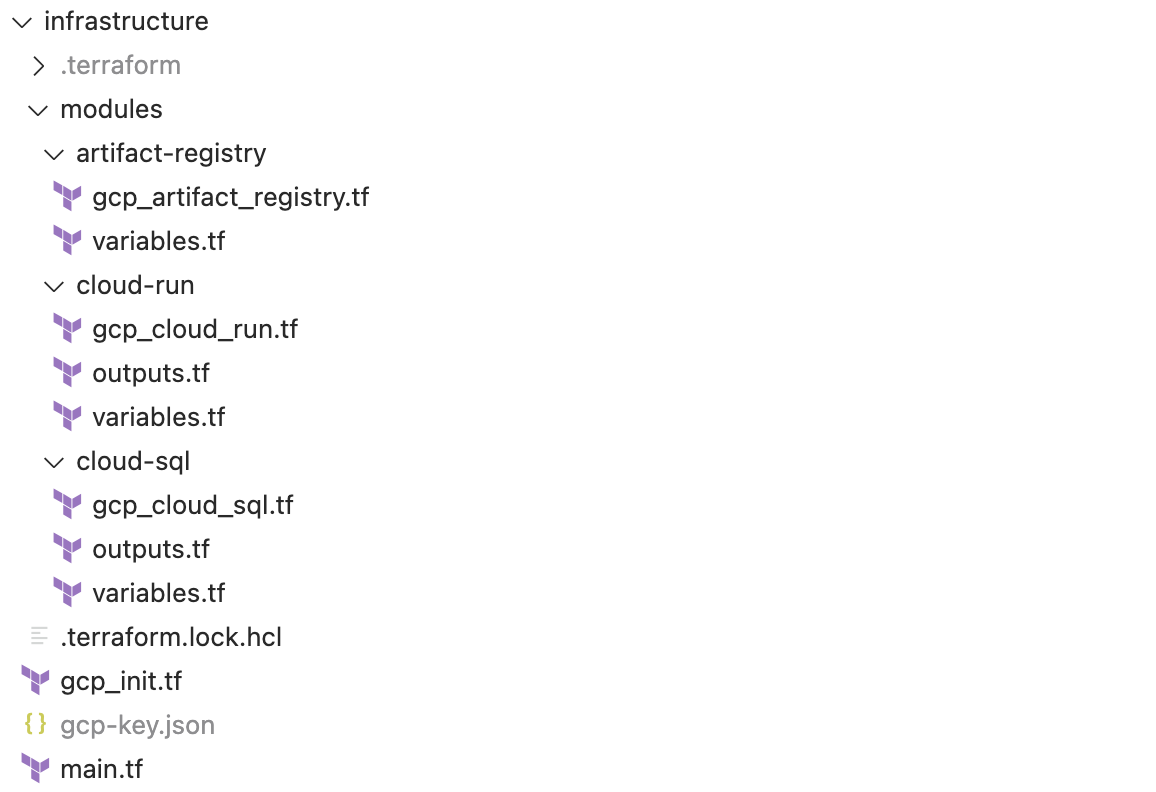
\includegraphics[scale=0.7]{filetree-infra}
\caption{The file tree of a fully functional infrastructure}
\label{fig:filetree-infra}
\end{figure}

Obviously, the implemented POC has numerous limitations.
This is the minimum amount of infrastructure needed to run the application without any encryption for the data.
The secrets are also not handled with a proper solution, as they are plaintext in the infrastructure code.
The routing is not handled to a custom domain either.
However, the application is now accessible to anyone on the internet and this counts as a minimum viable product (MVP) for the POC project specification, albeit without any security measures yet.

\section{Implementing encryption for the application}

In this section, the application and infrastructure built in the section before are improved by adding proper security measures.
We will add envelope encryption to the application and the infrastructure required by it.
The secret environment variables are also moved into GCP's Secret Manager for added security.

\subsection{Implementing envelope encryption in the TypeScript application}

Our encryption-specific code is placed inside \texttt{encryption.ts} file.
First, the application decrypts the key encryption key.
This is done via Google's own \\\texttt{@google-cloud/kms} npm-package. An example implementation is shown in Listing \ref{alg:decrypt-kek}.

\begin{algorithm}[htb]
\begin{minted}{typescript}
const kms = new KeyManagementServiceClient();
const ciphertextBuffer = Buffer.from(KEY_ENCRYPTION_KEY, "base64");
const keyName =
  kms.cryptoKeyPath("dippapoc", "global", KMS_KEYRING, KMS_KEY);
const [decryptResponse] = await kms.decrypt({
  name: keyName,
  ciphertext: ciphertextBuffer,
});
const { plaintext } = decryptResponse;
const keyEncryptionKey = Buffer.from(plaintext);
\end{minted}
\caption{An example implementation for decrypting the key encryption key with Cloud Key Management.}
\label{alg:decrypt-kek}
\end{algorithm}

Inside the \texttt{encrypt.ts} file, we also declare functions for generating, encrypting and decrypting pseudorandom data encryption keys, as well as functions for encrypting and decrypting data with any key provided.
The DEKs are generated using Node.js' built-in crypto-module's pseudorandom data generation via the \texttt{randomBytes}-function.
An example implementation for generating a key is shown in Listing \ref{alg:generate-datakey}.

\begin{algorithm}[htb]
\begin{minted}{typescript}
const generateDataKey = (): Buffer => {
  return crypto.randomBytes(32);
};
export { generateDataKey };
\end{minted}
\caption{An example implementation for generating a pseudorandom data encryption key.}
\label{alg:generate-datakey}
\end{algorithm}

For encrypting and decrypting data we will declare functions in the same file.
Encryption is done with the strong AES-256-CBC algorithm supported by the crypto-module.
Encrypting data is done using crypto-module's \texttt{createCipheriv}-function.
Decrypting data is done similary via the \texttt{createDecipheriv}-function.
An example implementation for implementing encryption and decryption is shown in Listing \ref{alg:encrypt-decrypt}.

\begin{breakablealgorithm}
\caption{An example implementation for AES-256-CBC encryption and decryption.}
\begin{minted}{typescript}
// previous code omitted.
const algorithm = "aes-256-cbc";
const initVector = Buffer.from(CRYPTO_INIT_VECTOR, "hex");
const encrypt = (key: Buffer, plaintext: string) => {
  const cipher = crypto.createCipheriv(algorithm, key, initVector);
  let ciphertext = cipher.update(plaintext, "utf-8", "base64");
  ciphertext +=  cipher.final("base64");
  return ciphertext;
};
const decrypt = (key: Buffer, ciphertext: string) => {
  const decipher =
    crypto.createDecipheriv(algorithm, key, initVector);
  let plaintext = decipher.update(ciphertext, "base64", "utf-8");
  plaintext += decipher.final("utf-8");
  return plaintext;
};
export { /* ... */ encrypt, decrypt };
\end{minted}
\label{alg:encrypt-decrypt}
\end{breakablealgorithm}

The \texttt{encrypt} and \texttt{decrypt} functions created above can be used as-is for encrypting and decrypting the DEKs.
We just need to pass the KEK as the parameter for key.
An example is shown in Listing \ref{alg:encrypt-dek}.

\begin{breakablealgorithm}
\caption{An example implementation for encrypting and decrypting data encryption keys.}
\begin{minted}{typescript}
// previous code omitted.
const encryptDataKey = (dataKey: Buffer): string => {
  const dataKeyString = dataKey.toString("hex");
  return encrypt(keyEncryptionKey, dataKeyString);
};
const decryptDataKey = (dataKey: string): Buffer => {
  const dataKeyString = decrypt(keyEncryptionKey, dataKey);
  return Buffer.from(dataKeyString, "hex");
};
export { /* ... */ encryptDataKey, decryptDataKey };
\end{minted}
\label{alg:encrypt-dek}
\end{breakablealgorithm}

Using the functions declared in the \texttt{encryption.ts}-file, it is possible to encrypt and decrypt any of our data objects and data encryption keys.
As an example for how the functions are used, Listing \ref{alg:encrypt-appointment} implements encryption and decryption for a practitioner-object.
The encryption is done very similarly for an appointment.

\begin{breakablealgorithm}
\caption{An example implementation for encrypting and decrypting a practitioner-object.}
\begin{minted}{typescript}
const encryptPractitioner = (
  practitioner: Practitioner
): EncryptedPractitioner => {
  const key = generateDataKey();
  // Encrypt personal data with the data key
  const firstnames = encrypt(key, practitioner.firstnames);
  const lastname = encrypt(key, practitioner.lastname);
  const education = encrypt(key, practitioner.education);
  // Wrap the data key with the key encryption key
  const data_key = encryptDataKey(key);
  return { firstnames, lastname, education, data_key };
};

const decryptPractitioner = (
  practitioner: EncryptedPractitioner
): Practitioner => {
  const { data_key, id } = practitioner;
  // Decrypt the data key with the key encryption key
  const key = decryptDataKey(data_key);
  // Use the data key to decrypt rest of the fields
  const firstnames = decrypt(key, practitioner.firstnames);
  const lastname = decrypt(key, practitioner.lastname);
  const education = decrypt(key, practitioner.education);
  return { firstnames, lastname, education, id };
};
\end{minted}
\label{alg:encrypt-appointment}
\end{breakablealgorithm}

% Voi myös miettiä, voiko koko ratkaisua/asetelmaa jotenkin esittää myös kuvallisesti
% -SR

\subsection{Implementing infrastructure for envelope encryption}

The application we now have requires new infrastructure to support envelope encryption: Google Cloud Key Management.
On top of adding a KMS key, we will move our secret environment variables such as database configuration and cryptographic secrets into GCP's Secret Manager.

To add Cloud Key Management to the POC application, we need three new resources managed by Terraform:
\begin{itemize}
    \item A KMS keyring to store cryptographic keys
    \item A KMS key to be used for cryptographic operations
    \item A KMS IAM member to update the IAM policy to allow Cloud Run to access it
\end{itemize}
An example implementation is shown in Listing \ref{alg:kms}.

\begin{breakablealgorithm}
\caption{An example implementation for adding Cloud Key Management infrastructure.}
\begin{minted}{terraform}
resource "google_kms_key_ring" "keyring" {
  name     = "dippapoc-keyring"
  location = "global"
}
resource "google_kms_crypto_key" "key" {
  name            = "dippapoc-key"
  key_ring        = google_kms_key_ring.keyring.id
  rotation_period = "2592000s" # 30 days
}

data "google_project" "project" {}
resource "google_kms_crypto_key_iam_member" "kms_compute" {
  crypto_key_id = google_kms_crypto_key.key.id
  role      = "roles/cloudkms.cryptoKeyDecrypter"
  member    = <<EOF
serviceAccount:${
  data.google_project.project.number
}-compute@developer.gserviceaccount.com
EOF
}
\end{minted}
\label{alg:kms}
\end{breakablealgorithm}

Adding the infrastructure for Secret Manager and the secrets themselves is handled by Terraform.
For a single secret that is accessible by Cloud Run, we need three new resources:
\begin{itemize}
    \item A Secret Manager Secret for a logical place to store a single secret
    \item A Secret Manager Secret version which holds the value of the secret itself
    \item A Secret Manager Secret IAM policy to allow Cloud Run to access the secret
\end{itemize}
For ease of use, these resources are bundled into a reusable module, which is called \texttt{./modules/secret} in the example.
Referencing the Secret Manager secrets as Cloud Run environment variables is not very different from referencing the values themselves.
To reference a Secret Manager secret with Terraform in a Cloud Run service config, a \texttt{value\_from} block is used.
An example of this is shown in Listing \ref{alg:secret-manager}.

\begin{breakablealgorithm}
\caption{An example implementation for referencing a Secret Manager secret in a Cloud Run service.}
\begin{minted}{terraform}
resource "google_cloud_run_service" "run_service" {
  name     = var.name
  location = "europe-north1"

  template {
    spec {
      containers {
        image = var.docker_image
        
        env {
          name  = "PGUSER"
          value = var.pguser # the value itself
        }
        env {
          name = "PGPASSWORD"
          value_from {
            secret_key_ref {
              name = var.secret_id_pgpassword # id of a secret
              key  = "latest"
            }
          }
        }
      }
    }
  }
}
\end{minted}
\label{alg:secret-manager}
\end{breakablealgorithm}

\chapter{The effect of encryption} \label{effect of encryption}

This chapter includes analysis on how adding encryption to a backend-application affects its complexity and performance.
The analysis is based on the POC project built for the thesis.

\section{The effect on complexity}

Adding extra features to any application obviously increases the complexity.
This complexity adds to the cost of maintaining the application, as the codebase gets larger and therefore harder to reason about.
There are options for dealing with the complexity, such as building abstractions that make reasoning with the program code on a higher level easier.
\cite{complexity-triggers}

\subsection{The effect on the complexity of the program code}

Adding envelope encryption to the program code and encrypting the database columns increases the complexity of the application.
Node.js’ crypto-module handles most of the encryption work, but interfacing with the Cloud Key Management is done using Google’s pre-made Npm-library which adds a dependency to manage.
A bit of additional configuration is required for accessing the GCP project as well as storing cryptographic secrets.

In the implemented POC project, the main encryption logic is abstracted into the \texttt{encryption.ts}-file, into only 6 functions.
This is quite a small amount of code to implement the encryption, which makes it easier to understand and maintain.
However, it still adds to the overall complexity of the application.

The design of the POC calls the encrypt and decrypt functions right at the service-level before or after accessing the database respectively.
The functions are called only on the sensitive fields, and not on database identifiers for example.
An example of this is shown in Listing \ref{alg:encrypt-appointment}.
This logic is not very complex, as the encryption itself is not implemented here, but it still requires adding quite a large amount of code.
The POC has no generic solution for encrypting any object, so an encrypt and decrypt function have to be created for each data type separately.

\subsection{The effect on the complexity of the infrastructure}

The addition of envelope encryption and storing the secrets required also increases the requirements of the infrastructure.
The two new Google Cloud services added are Cloud Key Management and Secret Manager.
Both of these also require IAM-configuration to allow our application to access them.

Cloud Key Management is a fully managed service, and not much configuration is required from the developer.
However, being an external API, it adds a possibility for an I/O bottleneck in our application.
This is why the POC application uses envelope encryption, only wrapping the key encryption key with the KMS.
Google Cloud’s documentation also suggests doing this. \cite{googlecloud}
The request-based pricing of KMS is also something that might affect very large applications.
Rotating the KMS keys is also something not implemented in the POC, which should be taken care of in a real world application.

Service Manager is another fully managed service which requires just as little configuration.
Only the secret, its data and IAM-configuration for the application are required.
Referencing the secrets in Cloud Run’s configuration is not a lot of added code either.
From the application’s point of view, it does not change anything where the environment variables are stored: the application accesses them the same way in either case.

\section{The effect on performance}

In this section, the fully built application's performance is tested.
The performance of the application is tested with both encryption enabled and disabled.
The goal is to measure the overhead caused by the encryption.

\subsection{Load testing}

Load testing refers to the practice of measuring a web application's quality of service performance.
The quality of service consists of two measures:
\begin{itemize}
    \item 
    \textit{Availability} – the percentage of times a customer is able to access the application
    \item 
    \textit{Response time} – the time it takes for the customer's action to be fulfilled.
\end{itemize}
Load testing from a single geographical location and during a single time window will not give you the complete picture.
End-to-end response time is dependent on a variety of things such as the user's location and the type of their network connection.
\cite{loadtesting}

Load testing can be used to predict a web application's performance at specific loads.
The load testing data can be further analysed to calculate the throughput of an application.
The throughput is a function of the number of concurrent requests and the stress on the system resources, most easily measured in request time.
\cite{loadtesting}

\subsection{The testing strategy}

To load test the POC application, we will first limit the scaling on the Cloud Run service to a maximum of one container.
This is done to observe changes in the stress level without needing equally as scalable tooling for running the load tests.
2000 simultaneous requests is enough to observe a difference in the performance of the application.
Under default settings, Cloud Run would activate more than 50 containers to support the load.

The testing will be conducted with Apache's JMeter: an application designed to load test and measure performance of many different applications/protocols.\footnote{Homepage of Apache JMeter: https://jmeter.apache.org/}
JMeter is configured to run 2000 simultaneous requests to the server and measure the response times.
The application is first built and deployed with encryption disabled, and then with encryption enabled.
Before each test, the database is cleared.
The test plan is to first call the \texttt{POST /practitioners/} endpoint 2000 times, adding the number of practitioners in to the database.
Second, we will call the \texttt{GET /practitioners/} endpoint 2000 times, fetching all of the practitioners each time.
Hypothesis for the results is that the added computation required by the encryption will cause an increase in response time and therefore a decrease in throughput.

\subsection{The results of the load testing}

The load test on the \texttt{POST /practitioners/} endpoint show a clear difference in both response time and throughput.
When encryption is enabled, the server takes almost a second longer to respond to begin with, and only slows from there.
While unencrypted, the response time does climb as the load increases, but the throughput still manages to go quite high before plateauing.
Both tests succeeded in all of the requests, so 100\% availability was achieved.
The visualization of the tests results is shown in Figure \ref{fig:post-practitioners}.

\begin{figure}[!htb]
\centering
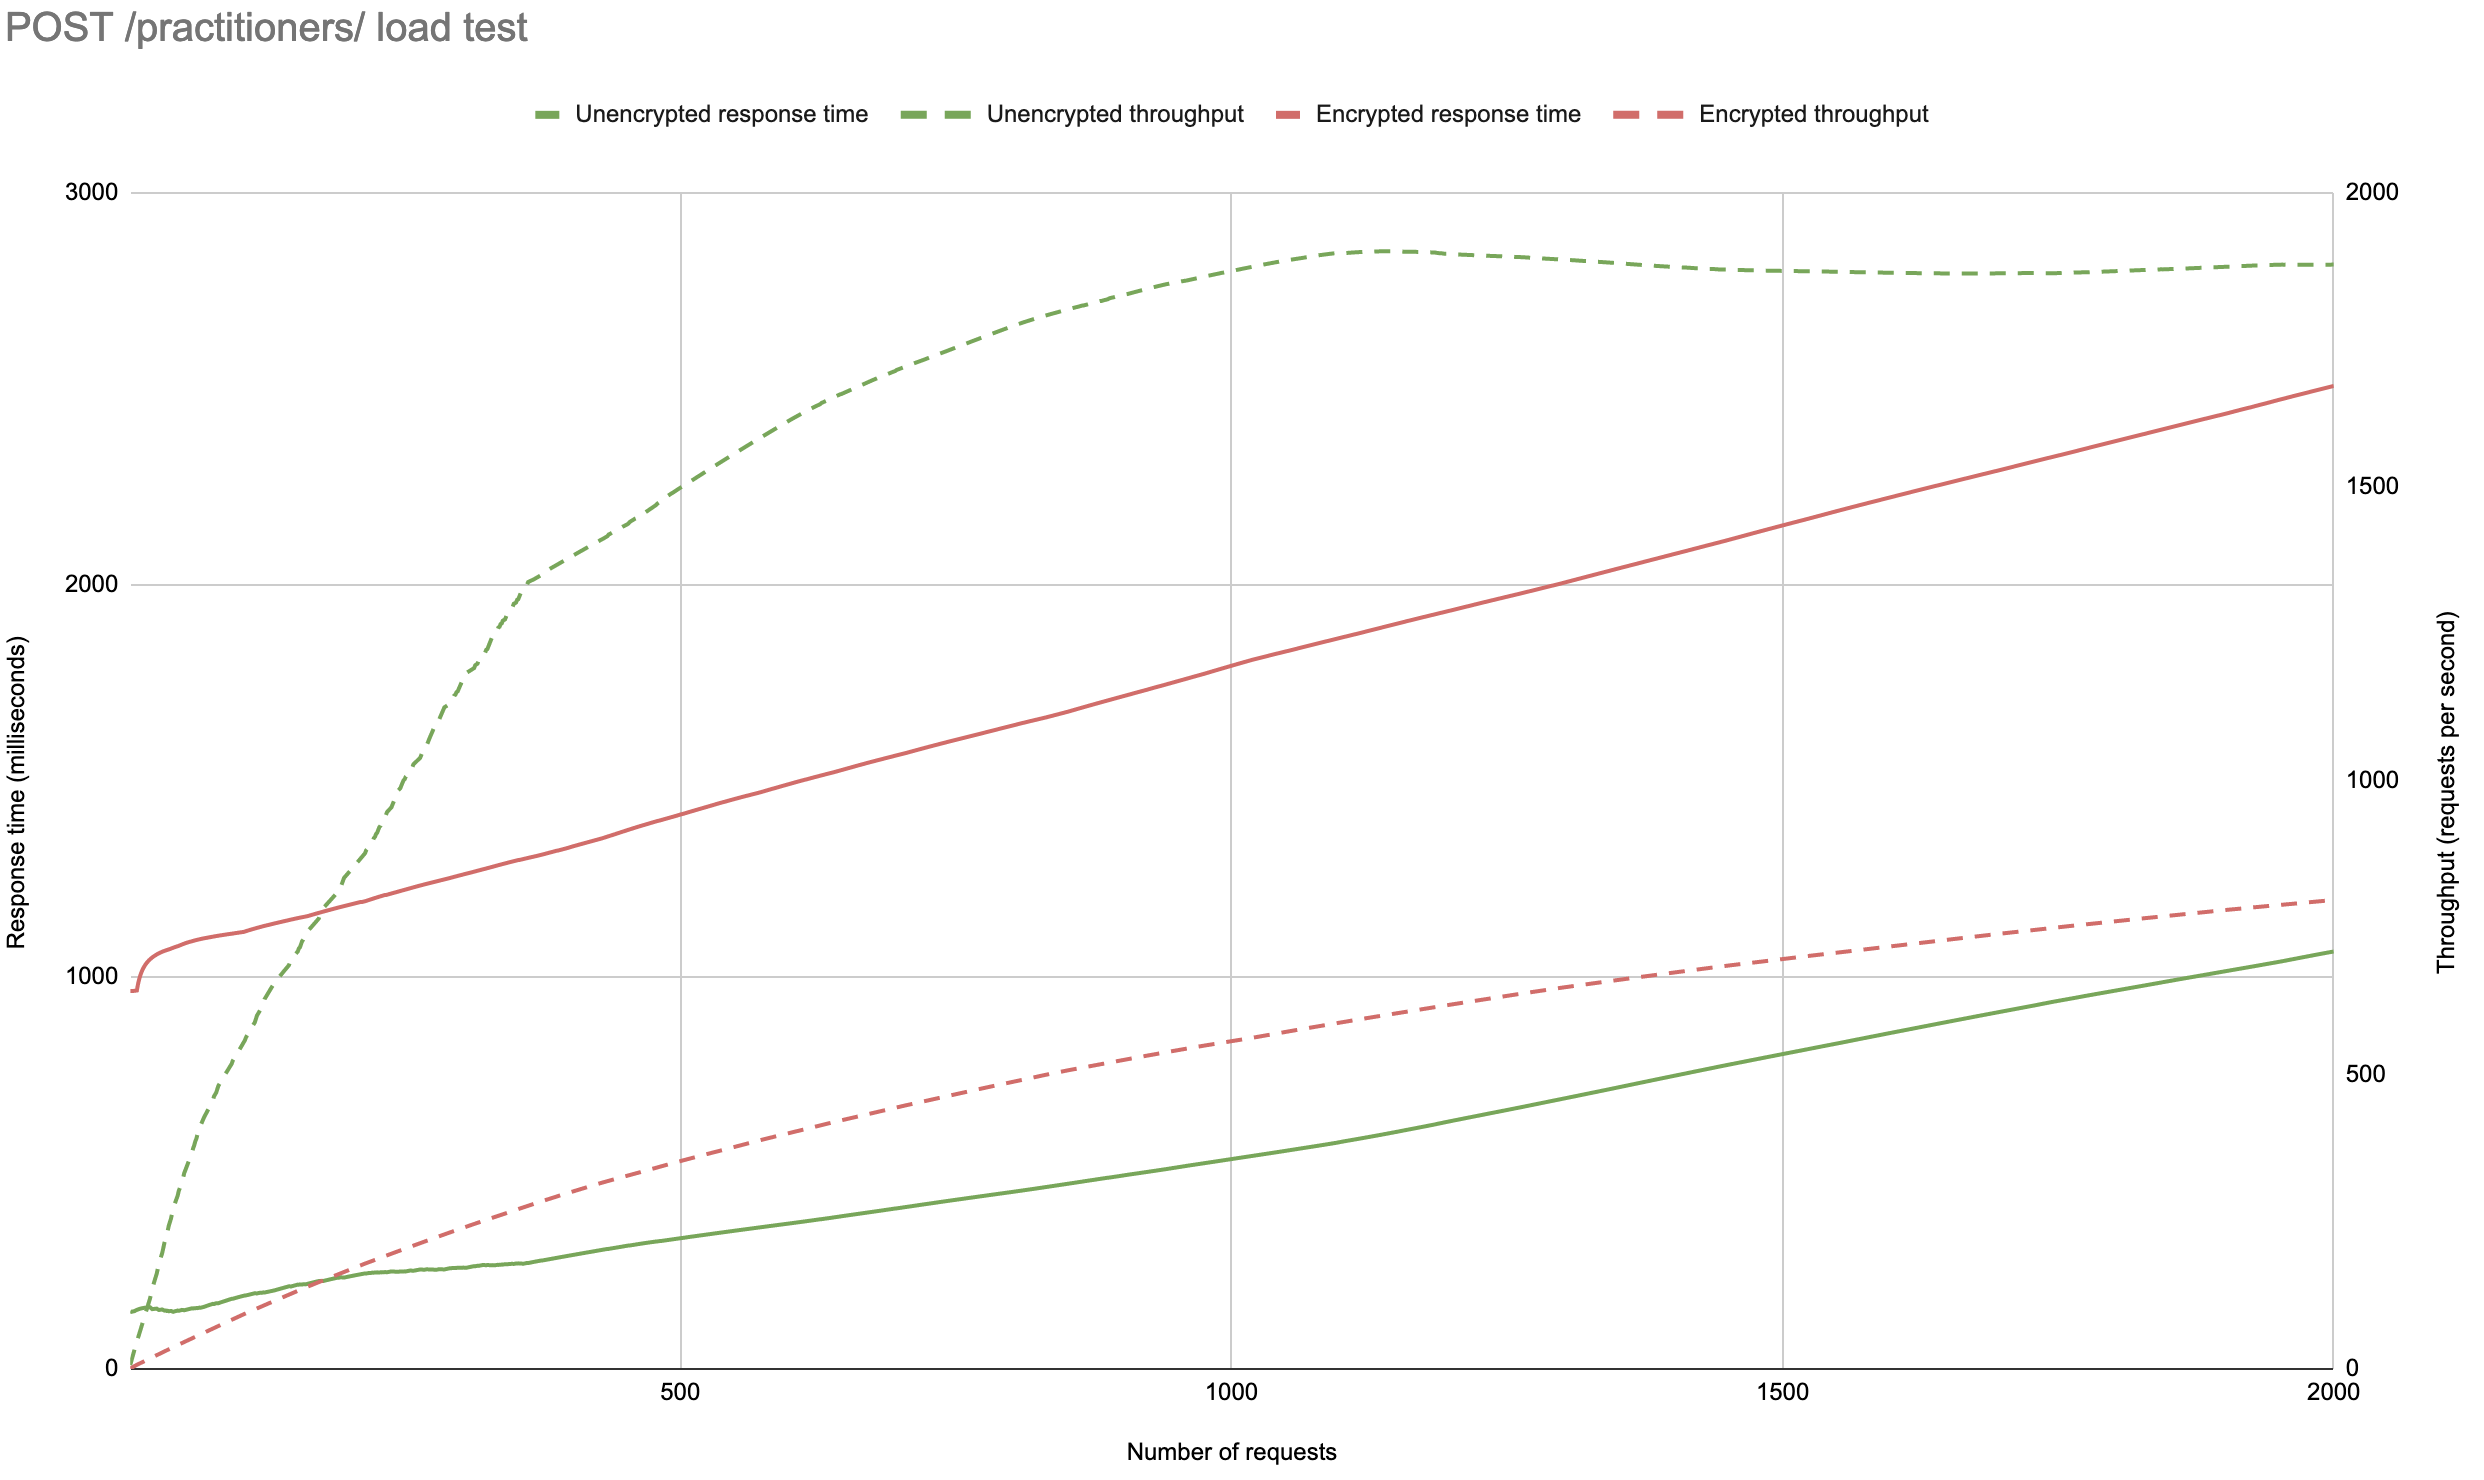
\includegraphics[scale=0.35]{post-practitioners}
\caption{POST /practitioners/ load test results.}
\label{fig:post-practitioners}
\end{figure}

The load tests on the \texttt{GET /practitioners/} endpoint show quite a different result.
At first, both encrypted and unencrypted take approximately the same time to respond to the request.
Both of the response times start climbing as the load increases, the encrypted response time spiking very sharply.
However, both of the response times plateau after enough load.
The encrypted application's response time plateauing around a hundred requests, and the unencrypted application's at around 500 requests.
This causes the throughput to start climbing instead.
The visualiztion of the tests results is shown in Figure \ref{fig:get-practitioners}.

\begin{figure}[!htb]
\centering
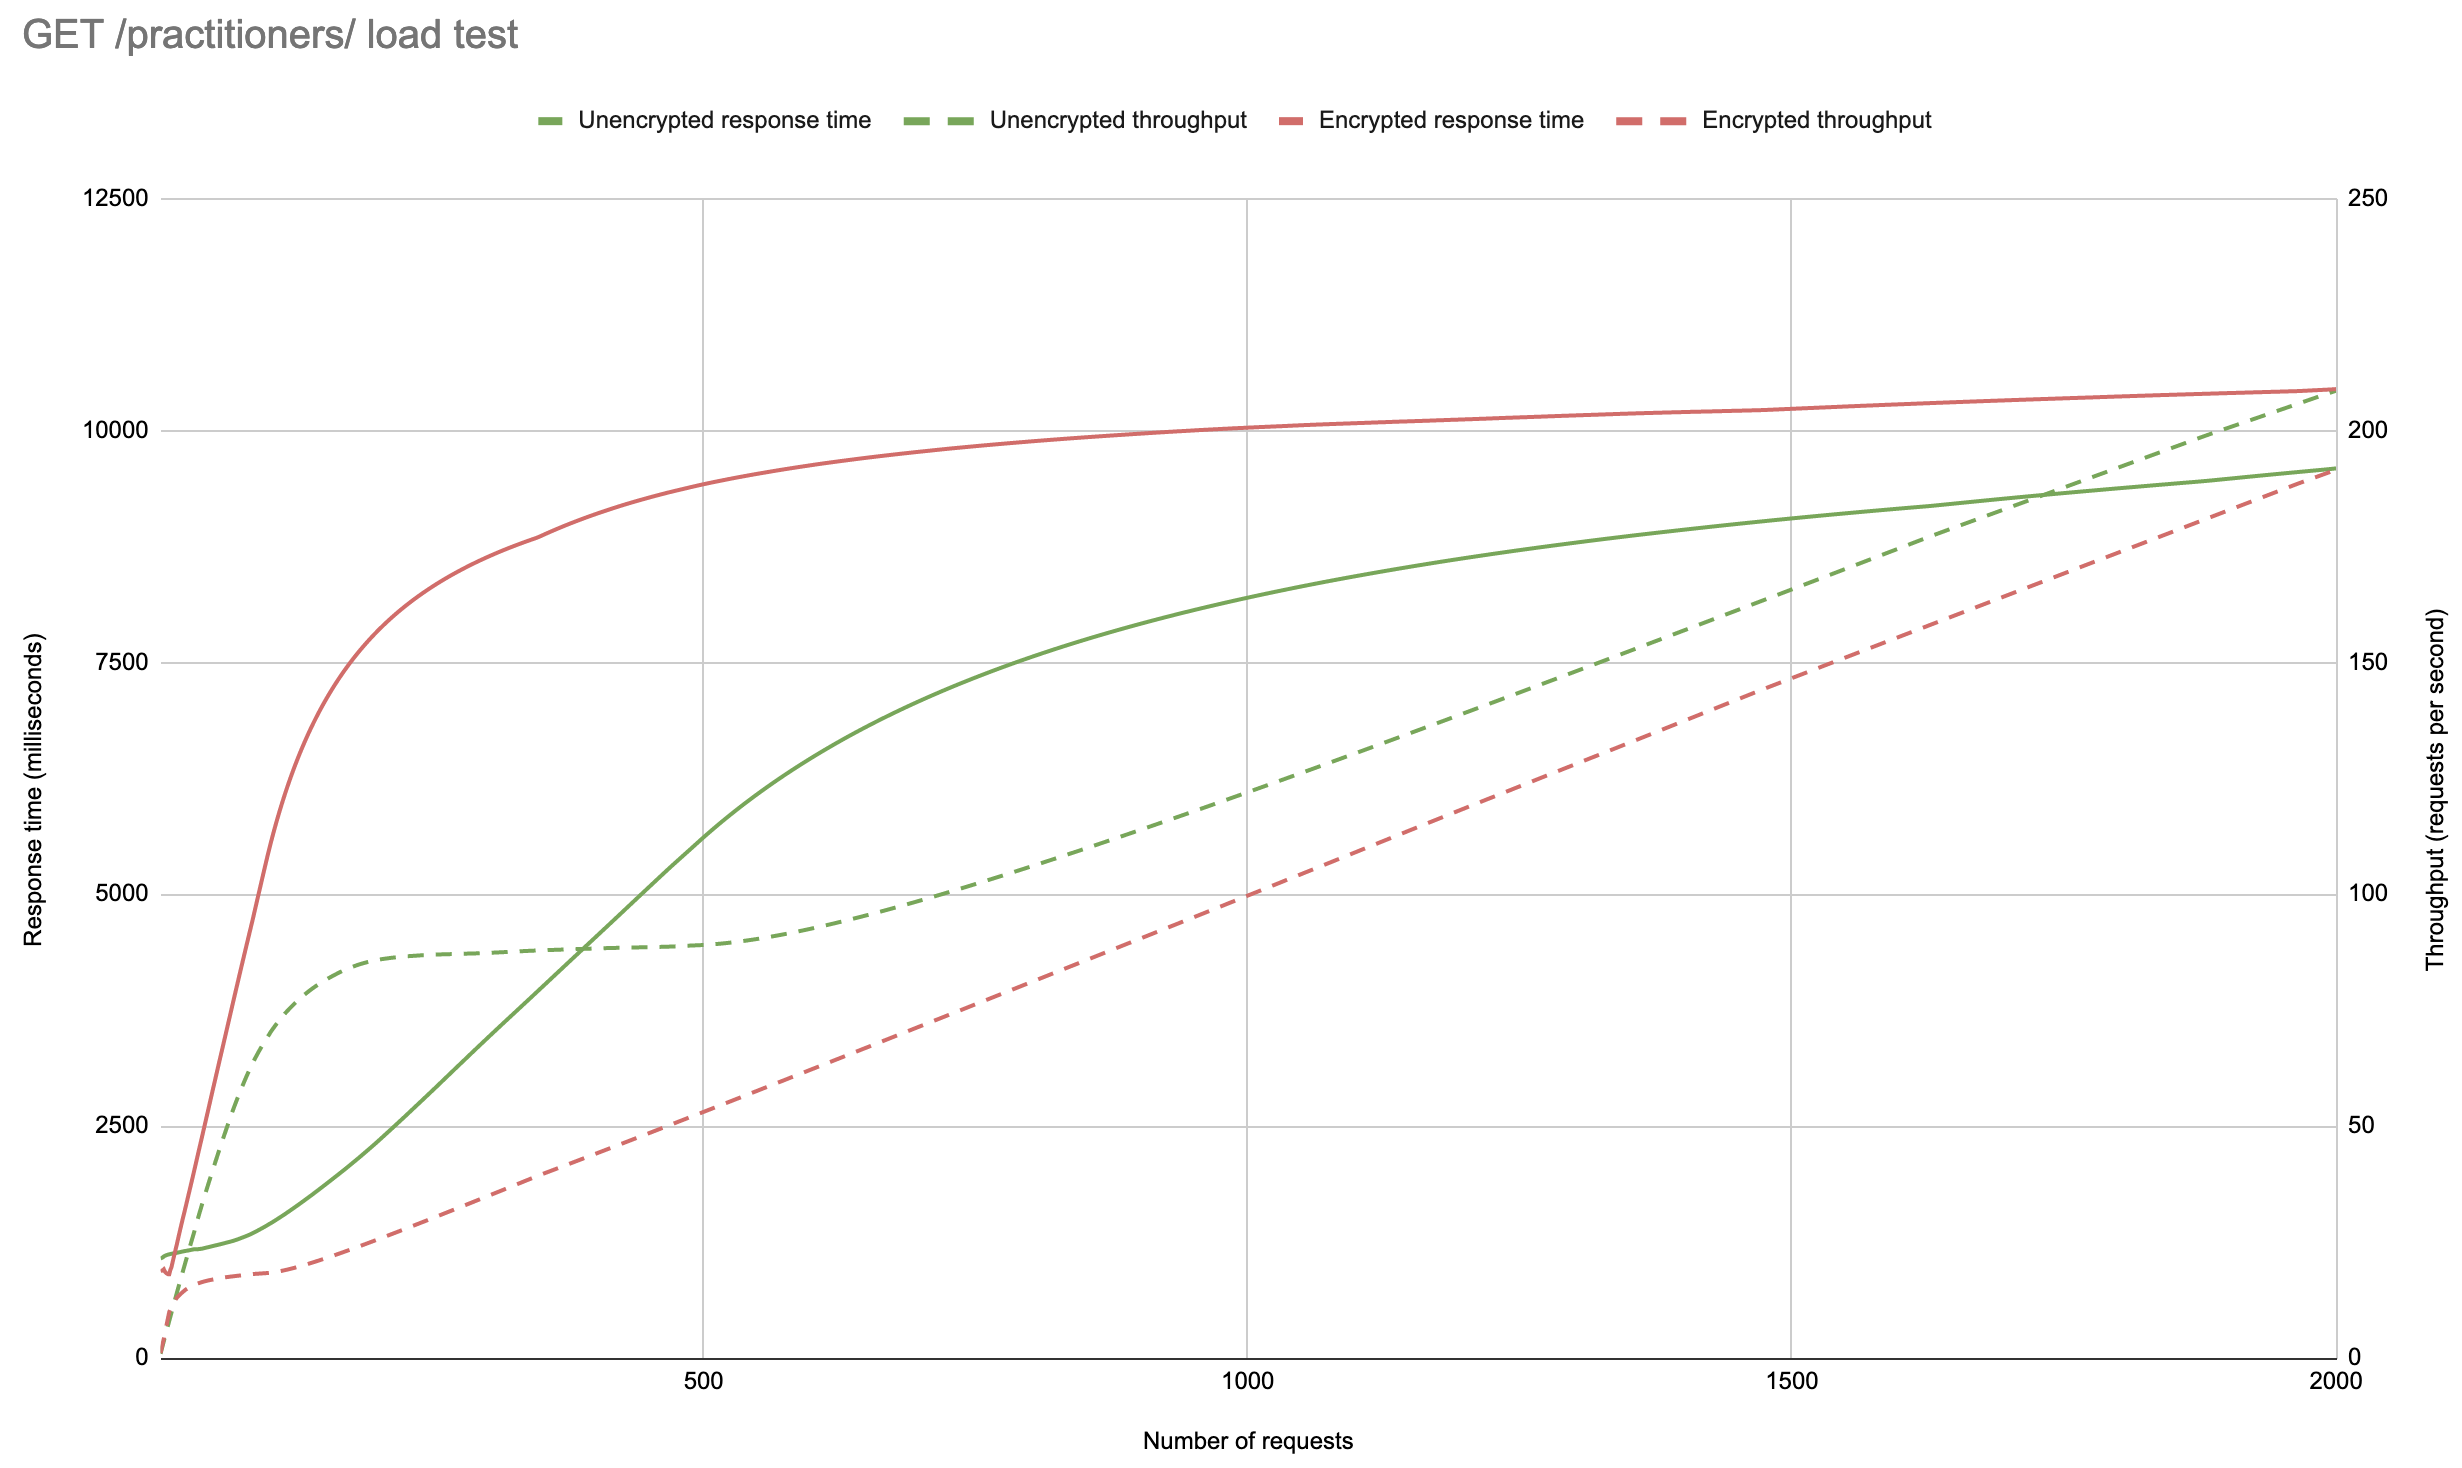
\includegraphics[scale=0.35]{get-practitioners}
\caption{GET /practitioners/ load test results.}
\label{fig:get-practitioners}
\end{figure}

The reason for the odd results for the \texttt{GET /practitioners/} endpoint is the success rate of the requests: the server starts refusing requests after enough load and responding with \texttt{HTTP 429 Too Many Requests} instead.
This means our application was not able to serve the load of 2000 simultaneous requests with 100\% availability.
The number of errors increasing as load increases is visualized in Figure \ref{fig:get-practitioners-errors}.

\begin{figure}[!htb]
\centering
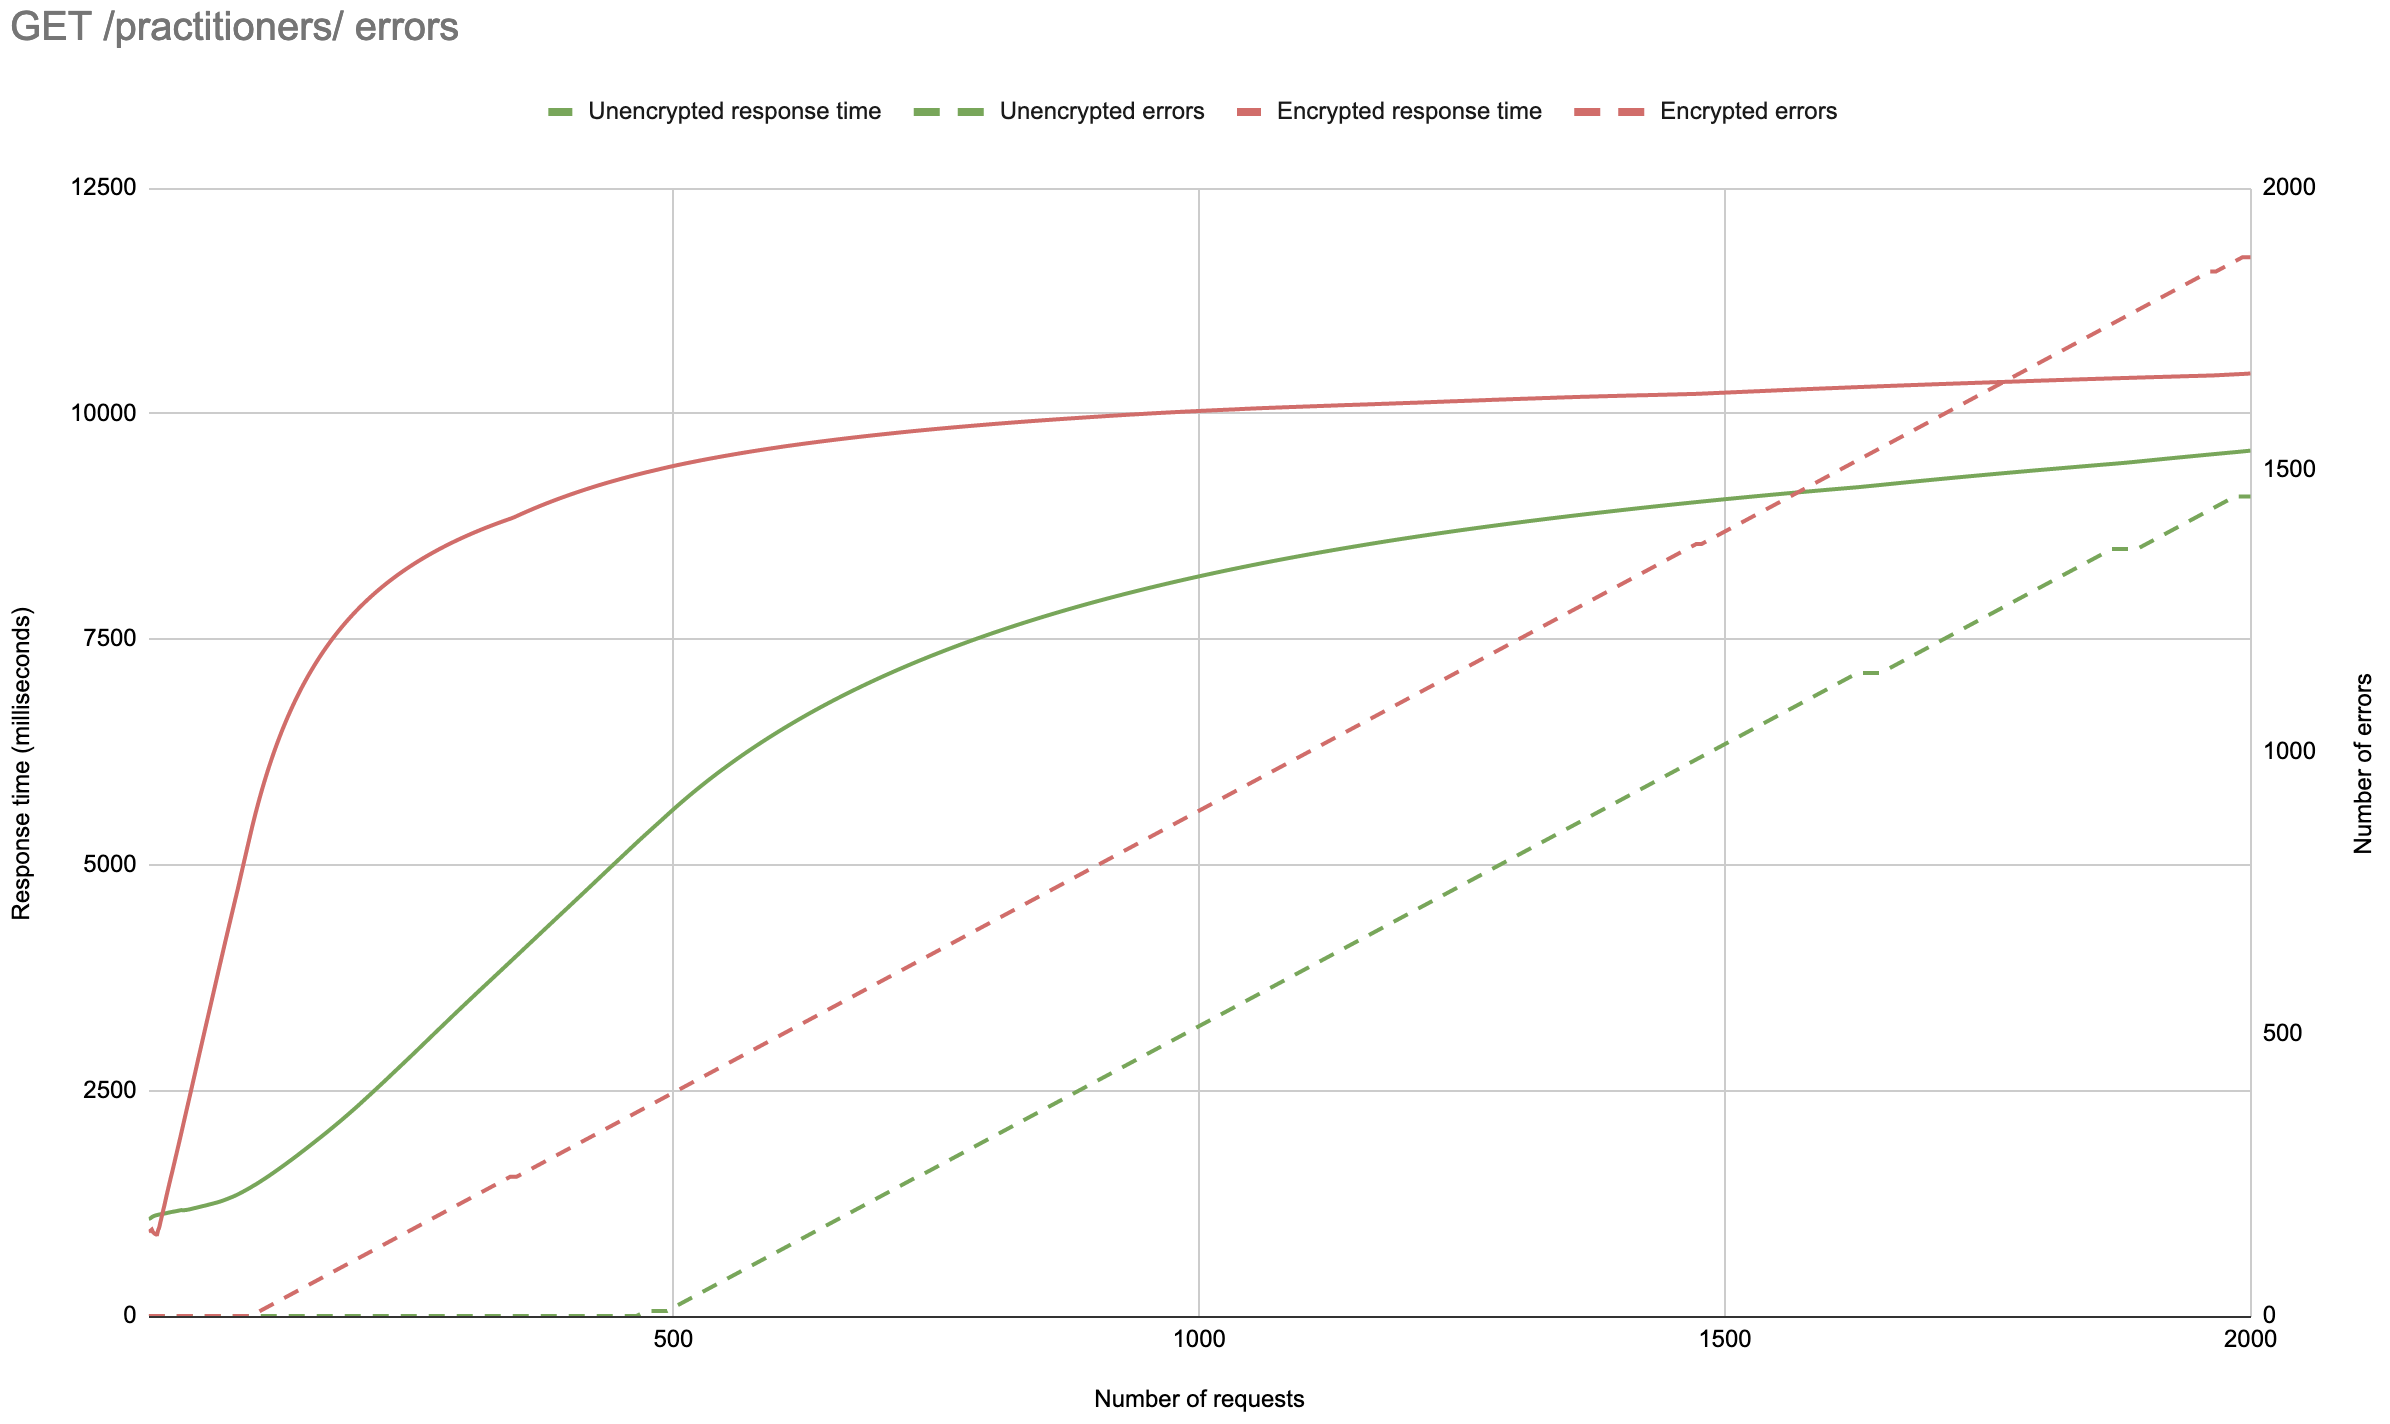
\includegraphics[scale=0.35]{get-practitioners-errors}
\caption{GET /practitioners/ response time and errors.}
\label{fig:get-practitioners-errors}
\end{figure}

The difference in the two endpoints' load tests is most likely caused by the large difference in the work required by each endpoint.
Namely, the amount of data passing through the application.
In the case of the \texttt{POST /practitioners/} endpoint, a single practitioner-object is sent to the server and stored in the database.
As for the \texttt{GET /practitioners/} endpoint, all of the practitioner-objects in the database have to be queried from the database and converted into JSON.

\section{Analysis}

The addition of encryption and its requirements on the infrastructure adds to the complexity of the application.
This added complexity will increase the cost of building and maintaining a similar application.
However, that complexity is largely dealt with by existing solutions available, such as the Cloud Key Management and Node.js' crypto-module used here.
No low-level knowledge of implementing cryptography is required by the developer, only enough to use the existing solutions securely.
Due to the laws in effect in Finland requiring proper security measures from all applications dealing with sensitive data, the added cost of this extra complexity should be taken into account when budgeting for such a project.

The hypothesis of encryption affecting performance negatively holds true.
However, the difference is not as large as expected.
Modern hardware is excellent at running encryption, and our application is most likely limited more by its I/O, rather than the extra computation required by the encryption.

The \texttt{GET /practitioners/} endpoint failing after some requests is not because of the encryption, as the unencrypted test was also affected by this.
The endpoint's functionality of loading an entire database table's data and sending it to the client is not a common real world use case.
Calling such an endpoint thousands of times simultaneously is certainly not a realistic scenario.

The POC project implemented leaves room for improvement in all of the fields tested.
Options for improving the design and implementation are discussed in the next chapter.

% \input{08-improving-performance}
\chapter{Conclusion} \label{conclusion}

The laws regarding storing individuals' private data in effect in Finland require additional technical knowledge and work from developers dealing with such data.
Healthcare organizations are forced to comply with the requirements and possibly implement additional security measures to their digital services.
The GDPR also adds extra measures to using a third party hosting provider.
Users of any public cloud provider have to take extra caution no third party can gain access to the sensitive data.
The individual must also be fully informed on where and how their data is stored and processed.

The GDPR and the Finnish law do not go into specifics regarding the technical implementation.
However, encryption and pseudonymization of data is encouraged to keep the data safe from a malicious actor.
These requirements have to be considered when implementing a digital service that stores any private data.

\section{The results of the research}

The proof-of-concept project built to mimic a real world healthcare service shows clear results on how encryption affects a cloud-based application's implementation and performance. Implementing encryption requires additional knowledge on cryptography from the development team.
However, the developer of a web application should almost never create and deploy their own cryptographic algorithm.\cite{dont-roll-crypto}
Libraries and tools exist for implementing encryption which should be preferred over custom cryptography implementations.
Nevertheless, implementing encryption will increase the complexity of the application.

In the case of the POC project created for this thesis, a lot of the complexity is handled by existing solutions such as Google Cloud Platform’s Cloud Key Management and Node.js’ built-in crypto-library.
However, implementing encryption increased the codebase size of both the application and the infrastructure by quite a bit.
This increased complexity makes the codebase harder to understand and therefore increases the cost to maintain it.

The added computation required by the encryption also affected the performance of the application.
Load testing shows a clear increase in response times when encryption is enabled.
Similarly, the throughput of the application decreased with encryption.
However, this difference between the two tests is not as large as it might be assumed.
The application is most likely more limited by its I/O.
The performance hit might still affect the costs of hosting the application in a public cloud.

\section{Options for improvement}

The POC project was built to mimic a real world healthcare service’s use case and implementation.
However, it is not feature-complete enough to be deployed in to the real world.
All the tested aspects of the application have room for improvement.

The security of the application could be further improved in a few different ways.
The data is only being kept safe from a third party gaining access to the database, as Google still has access to all the keys required to decrypt it.
This could be improved by storing any of the keys required to decrypt the data outside of the Google Cloud.

In the POC project, the key encryption key is stored inside program memory during runtime.
This responsibility could be moved to the Cloud Key Management by using its API to encrypt and decrypt the data encryption keys.
This would make it harder for a malicious actor to gain access to both, the KEK and the DEK.
In a real world use case, the KEK would also have to be rotated regularly, which was not considered in the POC implementation.
The secrets could also be handled separately from the Terraform configuration, making sure they are not committed to version control in either Terraform’s configuration or state files.

The added complexity of implementing encryption could also be handled better.
The application could use another layer of abstraction handling the encryption.
This abstraction could be implemented between the business logic and the database layer, making reasoning about the application logic on a high level easier without having to consider the underlying encryption.
The infrastructure configuration could separate encryption-specific configuration to its own modules.

The performance of the application can also be improved.
The application was found to handle 2000 simultaneous requests quite well while running in a single process.
The server application is stateless, which means it can natively scale into multiple processes in a fully managed service such as GCP’s Cloud Run.
The database’s performance has space for performance improvement as well -- perhaps by adding a fast in-memory cache.

The \texttt{GET /practitioners/} endpoint failing could be improved with a better design.
In a real world scenario, loading all the rows from an entire database table is not a good idea.
Instead, the client and the server should be designed to use pagination.
This reduces the bottleneck in loading data, as the data is not loaded all at once.

% The thesis main content ends here.

\printbibliography

\appchapter{Application code} \label{application-code}

\begin{breakablealgorithm}
    \caption{package.json}
    \inputminted{json}{app/package.json}
\end{breakablealgorithm}

\begin{breakablealgorithm}
\caption{tsconfig.json}
\inputminted{json}{app/tsconfig.json}
\end{breakablealgorithm}

\begin{breakablealgorithm}
\caption{docker-compose.yml}
\inputminted{yaml}{app/docker-compose.yml}
\end{breakablealgorithm}

\begin{breakablealgorithm}
\caption{Dockerfile}
\inputminted{Dockerfile}{app/Dockerfile}
\end{breakablealgorithm}

\begin{breakablealgorithm}
\caption{build.sh}
\inputminted{bash}{app/build.sh}
\end{breakablealgorithm}

\begin{breakablealgorithm}
\caption{sql/init.sql}
\inputminted{sql}{app/sql/init.sql}
\end{breakablealgorithm}

\begin{breakablealgorithm}
\caption{src/index.ts}
\inputminted{ts}{app/src/index.ts}
\end{breakablealgorithm}

\begin{breakablealgorithm}
\caption{src/config.ts}
\inputminted{ts}{app/src/config.ts}
\end{breakablealgorithm}

\begin{breakablealgorithm}
\caption{src/db.ts}
\inputminted{ts}{app/src/db.ts}
\end{breakablealgorithm}

\begin{breakablealgorithm}
\caption{src/encryption.ts}
\inputminted{ts}{app/src/encryption.ts}
\end{breakablealgorithm}

\begin{breakablealgorithm}
\caption{src/practitioner/practitionerController.ts}
\inputminted{ts}{app/src/practitioner/practitionerController.ts}
\end{breakablealgorithm}

\begin{breakablealgorithm}
\caption{src/practitioner/practitionerTypes.ts}
\inputminted{ts}{app/src/practitioner/practitionerTypes.ts}
\end{breakablealgorithm}

\begin{breakablealgorithm}
\caption{src/practitioner/practitionerValidator.ts}
\inputminted{ts}{app/src/practitioner/practitionerValidator.ts}
\end{breakablealgorithm}

\begin{breakablealgorithm}
\caption{src/practitioner/practitionerService.ts}
\inputminted{ts}{app/src/practitioner/practitionerService.ts}
\end{breakablealgorithm}

\begin{breakablealgorithm}
\caption{src/appointment/appointmentController.ts}
\inputminted{ts}{app/src/appointment/appointmentController.ts}
\end{breakablealgorithm}

\begin{breakablealgorithm}
\caption{src/appointment/appointmentTypes.ts}
\inputminted{ts}{app/src/appointment/appointmentTypes.ts}
\end{breakablealgorithm}

\begin{breakablealgorithm}
\caption{src/appointment/appointmentValidator.ts}
\inputminted{ts}{app/src/appointment/appointmentValidator.ts}
\end{breakablealgorithm}

\begin{breakablealgorithm}
\caption{src/appointment/appointmentService.ts}
\inputminted{ts}{app/src/appointment/appointmentService.ts}
\end{breakablealgorithm}
\appchapter{Infrastructure code} \label{infrastructure-code}

\begin{breakablealgorithm}
\caption{gcp\_init.tf}
\inputminted{tf}{infrastructure/gcp_init.tf}
\end{breakablealgorithm}

\begin{breakablealgorithm}
\caption{main.tf}
\inputminted{tf}{infrastructure/main.tf}
\end{breakablealgorithm}

\begin{breakablealgorithm}
\caption{modules/secret/gcp\_secret\_manager\_secret.tf}
\inputminted{tf}{infrastructure/modules/secret/gcp_secret_manager_secret.tf}
\end{breakablealgorithm}

\begin{breakablealgorithm}
\caption{modules/secret/variables.tf}
\inputminted{tf}{infrastructure/modules/secret/variables.tf}
\end{breakablealgorithm}

\begin{breakablealgorithm}
\caption{modules/secret/outputs.tf}
\inputminted{tf}{infrastructure/modules/secret/outputs.tf}
\end{breakablealgorithm}

\begin{breakablealgorithm}
\caption{modules/cloud-run/gcp\_cloud\_run.tf}
\inputminted{tf}{infrastructure/modules/cloud-run/gcp_cloud_run.tf}
\end{breakablealgorithm}

\begin{breakablealgorithm}
\caption{modules/cloud-run/variables.tf}
\inputminted{tf}{infrastructure/modules/cloud-run/variables.tf}
\end{breakablealgorithm}

\begin{breakablealgorithm}
\caption{modules/cloud-run/outputs.tf}
\inputminted{tf}{infrastructure/modules/cloud-run/outputs.tf}
\end{breakablealgorithm}

\begin{breakablealgorithm}
\caption{modules/cloud-sql/gcp\_cloud\_sql.tf}
\inputminted{tf}{infrastructure/modules/cloud-sql/gcp_cloud_sql.tf}
\end{breakablealgorithm}

\begin{breakablealgorithm}
\caption{modules/cloud-sql/variables.tf}
\inputminted{tf}{infrastructure/modules/cloud-sql/variables.tf}
\end{breakablealgorithm}

\begin{breakablealgorithm}
\caption{modules/cloud-sql/outputs.tf}
\inputminted{tf}{infrastructure/modules/cloud-sql/outputs.tf}
\end{breakablealgorithm}

\begin{breakablealgorithm}
\caption{modules/artifact-registry/gcp\_artifact\_registry.tf}
\inputminted{tf}{infrastructure/modules/artifact-registry/gcp_artifact_registry.tf}
\end{breakablealgorithm}

\begin{breakablealgorithm}
\caption{modules/artifact-registry/variables.tf}
\inputminted{tf}{infrastructure/modules/artifact-registry/variables.tf}
\end{breakablealgorithm}

\begin{breakablealgorithm}
\caption{modules/key-management/gcp\_kms.tf}
\inputminted{tf}{infrastructure/modules/key-management/gcp_kms.tf}
\end{breakablealgorithm}

\begin{breakablealgorithm}
\caption{modules/key-management/variables.tf}
\inputminted{tf}{infrastructure/modules/key-management/variables.tf}
\end{breakablealgorithm}

\begin{breakablealgorithm}
\caption{modules/key-management/outputs.tf}
\inputminted{tf}{infrastructure/modules/key-management/outputs.tf}
\end{breakablealgorithm}


\end{document}
